% This is LLNCS.DEM the demonstration file of
% the LaTeX macro package from Springer-Verlag
% for Lecture Notes in Computer Science,
% version 2.4 for LaTeX2e as of 16. April 2010
%
\documentclass{llncs}

% allows for temporary adjustment of side margins
\usepackage{chngpage}

% just makes the table prettier (see \toprule, \bottomrule, etc. commands below)
\usepackage{booktabs}

\usepackage[utf8]{inputenc}
%\usepackage[font=small,skip=0pt]{caption}

% footnotes
\usepackage{scrextend}

% URL handling
\usepackage{url}
\urlstyle{same}

% Todos
%\usepackage[colorinlistoftodos]{todonotes}
%\newcommand{\ke}[1]{\todo[size=\small, color=orange!40]{\textbf{Kai:} #1}}
%\newcommand{\tb}[1]{\todo[size=\small, color=green!40]{\textbf{Thomas:} #1}}


%\usepackage{makeidx}  % allows for indexgeneration

%\usepackage{amsmath}
\usepackage{amsmath, amssymb}
\usepackage{mathabx}

% monospace within text
\newcommand{\ms}[1]{\texttt{#1}}

% examples
\usepackage{fancyvrb}
\DefineVerbatimEnvironment{ex}{Verbatim}{numbers=left,numbersep=2mm,frame=single,fontsize=\scriptsize}

\usepackage{xspace}
% Einfache und doppelte Anfuehrungszeichen
\newcommand{\qs}{``} 
\newcommand{\qe}{''\xspace} 
\newcommand{\sqs}{`} 
\newcommand{\sqe}{'\xspace} 

% checkmark
\usepackage{tikz}
\def\checkmark{\tikz\fill[scale=0.4](0,.35) -- (.25,0) -- (1,.7) -- (.25,.15) -- cycle;} 

% Xs
\usepackage{pifont}

% Tabellenabstände kleiner
\setlength{\intextsep}{10pt} % Vertical space above & below [h] floats
\setlength{\textfloatsep}{10pt} % Vertical space below (above) [t] ([b]) floats
% \setlength{\abovecaptionskip}{0pt}
% \setlength{\belowcaptionskip}{0pt}

\usepackage{tabularx}
\newcommand{\hr}{\hline\noalign{\smallskip}} % für die horizontalen linien in tabellen

% Todos
\usepackage[colorinlistoftodos]{todonotes}
\newcommand{\ke}[1]{\todo[size=\small, color=orange!40]{\textbf{Kai:} #1}}
\newcommand{\tb}[1]{\todo[size=\small, color=green!40]{\textbf{Thomas:} #1}}
\newcommand{\er}[1]{\todo[size=\small, color=red!40]{\textbf{Erman:} #1}}
\newcommand{\an}[1]{\todo[size=\small, color=blue!40]{\textbf{Andy:} #1}}

\newenvironment{table-1cols}{
  \scriptsize
  \sffamily
  \vspace{0.3cm}
  \begin{tabular}{l}
  \hline
  \textbf{Requirements} \\
  \hline

}{
  \hline
  \end{tabular}
  \linebreak
}

\newenvironment{table-2cols}{
  \scriptsize
  \sffamily
  \vspace{0.3cm}
  \begin{tabular}{l|l}
  \hline
  \textbf{Requirements} & \textbf{Covering DSCLs} \\
  \hline

}{
  \hline
  \end{tabular}
  \linebreak
}

\newenvironment{complexity}{
  %\scriptsize
  %\sffamily
  %\vspace{0.3cm}
  \begin{tabular}{l|l}
  \hline
  \textbf{Complexity Class} & \textbf{Complexity} \\
  \hline

}{
  \hline
  \end{tabular}
  \linebreak
}

\newenvironment{DL}{
  %\scriptsize
  %\sffamily
  \vspace{0cm}
  \begin{tabular}{r l}

}{
  \end{tabular}
  %\linebreak
}


\newenvironment{evaluation}{
  %\scriptsize
  %\sffamily
  %\vspace{0.3cm}
  \begin{tabular}{l|c|c|c|c|c|c}
  \hline
  \textbf{Constraint Class} & \textbf{DSP} & \textbf{OWL2-DL} & \textbf{OWL2-QL} & \textbf{ReSh} & \textbf{ShEx} & \textbf{SPIN} \\
  \hline

}{
  \hline
  \end{tabular}
  \linebreak
}

\newenvironment{constraint-languages-complexity}{
  %\scriptsize
  %\sffamily
  %\vspace{0.3cm}
  \begin{tabular}{l|c|c|c|c|c|c}
  \hline
  \textbf{Complexity Class} & \textbf{DSP} & \textbf{OWL2-DL} & \textbf{OWL2-QL} & \textbf{ReSh} & \textbf{ShEx} & \textbf{SPIN} \\
  \hline

}{
  \hline
  \end{tabular}
  \linebreak
}

\newenvironment{user-fiendliness}{
  %\scriptsize
  %\sffamily
  %\vspace{0.3cm}
  \begin{tabular}{l|c|c|c|c|c}
  \hline
  \textbf{criterion} & \textbf{DSP} & \textbf{OWL2} & \textbf{ReSh} & \textbf{ShEx} & \textbf{SPIN} \\
  \hline

}{
  \hline
  \end{tabular}
  \linebreak
}

\setcounter{secnumdepth}{5}

\begin{document}

%
%
\title{The Role of Constraint Languages and Reasoning for RDF Validation}
\subtitle{}
% On Constraint Languages for RDF Validation with an account to Reasoning
%On Constraint Languages for RDF Validation and Reasoning
%RDF Validation - Classification of Constraints and Constraint Languages According to Reasoning, Expressivity, and Complexity
%RDF Validation: An Analysis of Constraint Languages
%Analysing Constraint Languages for RDF Validation
%Classifying Constraint Languages for RDF Validation
%RDF Validation and Reasoning.
%Classifying Constraint Languages for RDF validation Concerning Reasoning
\titlerunning{XXXXX}  % abbreviated title (for running head)
%                                     also used for the TOC unless
%                                     \toctitle is used
%
\author{Thomas Bosch\inst{1} \and Erman Acar\inst{2} \and Andreas Nolle\inst{3} \and Kai Eckert\inst{2}}
%
\authorrunning{} % abbreviated author list (for running head)
%
%%%% list of authors for the TOC (use if author list has to be modified)
\institute{GESIS – Leibniz Institute for the Social Sciences, Germany\\
\email{thomas.bosch@gesis.org},\\ 
\and
University of Mannheim, Germany \\
\email{\{erman,kai\}@informatik.uni-mannheim.de} 
\and
Albstadt-Sigmaringen University, Germany \\
\email{nolle@hs-albsig.de}
}

\maketitle              % typeset the title of the contribution

\begin{abstract}

For data practitioners embracing the world of RDF and Linked Data, the openness and flexibility is a mixed blessing. For them, data validation according to predefined constraints is a  much sought-after feature, particularly as this is taken for granted in the XML world. Several approaches exist to meet this requirement, ranging from using OWL as a constraint language to SPIN, a SPARQL-based way to formulate and check constraints. There are also specific constraint languages like Shape Expressions, Resource Shapes or Description Set Profiles that more or less explicitly address the aforementioned data practitioners.
In this paper, we investigate the relationship of validation and reasoning and the role that reasoning plays in practical data validation. We formulate common types of constraints in Description Logic and use this formulation to determine their complexity when certain reasoning steps are involved. At last, we aggregate these findings for the most common constraint languages and show their commonalities and differences regarding constraint expressivity. We argue that so far no single best solution exists and that the results presented in this paper are crucial for a proper application of RDF validation.


% There is no standard way to formulate RDF constraints for validation,
% however there are several popular constraint languages (i.e., SPIN, ReSh, ShEx) covering major requirements on RDF validation. Amongst others, the ontology language OWL 2 can also be considered as an expressive constraint language with a high level human-readable syntax.
% In this work, we discuss possible scenarios on how OWL 2 reasoning can actually be useful for RDF validation.

%%We take reasoning into account as a possible pre-validation step, 
%%(1) to infer triples resolving constraint violations, 
%%(2) to infer triples for which constraints can also be validated, and 
%%(3) to solve the major shortcoming of RDF validation: redundancy. 
%%\er{I simplified the long abstract a bit by commenting (\%) as well as little editing. The part starting with, "we investigate", cause lacking integrity in abstract,  I dropped 1, 2, 3 for simplification and better flow. We can write abstract in the end, which can also include a short part of introduction if necessary.}

% Then, regarding a collected list of constraint types (requirements), we classify their expressivity with an account to reasoning.   

%%Following this approach, one can clarify which constraint language to use to express constraints for specific validation scenarios, with and without reasoning.
%%Validators can determine which axioms cause high complexity and which constraints can only be expressed within a more sophisticated expressivity class.
%%As a next step, validators give some guidance how to get to lower expressivity and complexity classes.
%%If validators propose multiple constraint languages for a particular validation use case, additional rather subjective criteria regarding user-friendliness may be evaluated.

\keywords{RDF Validation, RDF Constraints, OWL 2, Reasoning, RDF Validation Requirements, Linked Data, Semantic Web}
\end{abstract}
%

%\section{Possible Titles}
%
%keywords as part of the title
%
%\begin{itemize}
	%\item Classification of Constraint Languages 
	%\item Expressivity
	%\item Complexity
	%\item user-friendliness
	%\item RDF Validation
	%\item reasoning
	%\item Choosing Your RDF Constraint Language According to Expressivity, Complexity, and User-Friendliness
	%\item OWL 2 as Constraint Language for RDF Validation
	%\item Classification of RDF Validation Constraint Languages According to Expressivity, Complexity, and User-Friendliness 
	%\item RDF Validation - Classification of Constraint Languages According to Expressivity, Complexity, and User-Friendliness 
	%\item RDF Validation - Effects on Complexity with and without OWL 2 Reasoning
	% RDF Validation - Proposing / Comparing / Recommendation / Recommending Constraint Languages According to Expressivity, Complexity, and User-Friendliness
	% Constraint Validation with OWL 2
	% Constraint Validation with and without OWL
%\end{itemize}

\section{Introduction}

% How research about RDF validation started
% -----
%For many RDF applications, the formulation of constraints and the automatic validation of data according to these constraints is a much sought-after feature. 
In 2013, the W3C invited experts from industry, government, and academia to the RDF Validation Workshop\footnote{\url{http://www.w3.org/2012/12/RDF-val/}}, 
where first use cases on RDF validation have been presented and discussed. 
Two working groups (WGs) that follow up on this workshop and address RDF constraint formulation and validation, are established in 2014: 
the W3C RDF Data Shapes WG\footnote{\url{http://www.w3.org/2014/rds/charter}} and the DCMI RDF Application Profiles WG\footnote{\url{http://wiki.dublincore.org/index.php/RDF-Application-Profiles}}. 
% RDF validation requirements database
% -----
As a part of our earlier work \cite{BoschEckert2014}, we initiated a comprehensive database (publicly available at \url{http://purl.org/net/RDF-validation}) on RDF validation requirements to collect case studies, use cases, and requirements. It is continuously updated and used to evaluate and to compare various existing solutions for RDF constraint formulation and validation. 
Requirements are classified to provide a high-level view on different solutions and to facilitate a better understanding of the problem domain.  


% RDF validation in the library domain
% -----
Rdf validation gained speed as a research field in recent years, as a result of common needs.  For instance, libraries are used to publish data in form of XML documents for a long time.
They model and validate data using quite complex and very detailed XML Schemas, DTDs, RELAX NG, or Schematron.
Recently, libraries started to publish RDF data sets, since libraries have many use cases which are met by Semantic Web technologies and Linked Data. 
A library wants to publish some data sets as RDF by extracting them from different relational databases. 
In order to achieve high data quality some constraints are defined first on a very
generic level written down in some natural language sentences.  
Now it needs to be decided which formalism to use in order to formally express
these constraints and to check their validity. 
It is often needed to declare properties of given classes as mandatory.  
Publications, for instance, must have publishing dates.
Another common constraint is that literals of particular properties (e.g., ISBN identifiers) must correspond to some pattern.

% constraint languages
% -----
For expressing RDF constraints, there are numerous constraint languages, each with its own syntax and semantics.  
Yet none of them is an all-purpose standard, the most popular ones are
the SPARQL Inferencing Notation (SPIN)\footnote{\url{http://spinRDF.org/}} (representing SPARQL queries in RDF), 
the Web Ontology Language (OWL 2)\footnote{\url{http://www.w3.org/TR/owl2-syntax/}}, 
Shape Expressions (ShEx)\footnote{\url{http://www.w3.org/Submission/shex-primer/}}, 
Resource Shapes (ReSh)\footnote{\url{http://www.w3.org/Submission/shapes/}}, 
and Description Set Profiles (DSP)\footnote{\url{http://dublincore.org/documents/2008/03/31/dc-dsp/}}.
Their relevance varies with respect to several foremost criteria in the validation process, such as constraint expressivity (\emph{what kind of constraints can be expressed?}), performance (\emph{how efficient in terms of runtime can RDF data be validated?}), as well as intuitiveness and conciseness (\emph{how easy is it for a user to define constraints?}). 
%Furthermore, the service of reasoning and its usability is in question. 



% Reasoning
% - describe reasoning in general
% - why is reasoning important for validation?
% -----


%Reasoning is the process of determining what follows from what has been
%stated.

A major shortcoming when validating RDF data is redundancy.
\emph{Reasoning} seems to be a promising solution as pre-validation step to overcome this shortcoming. Reasoning (logical) is used in order to make the implicit knowledge explicit  {e.g., \emph{modus ponens}, books are publications, \em Foundations of Semantic Web Technologies} is a book, and therefore it is a publication) in many different forms. 
Reasoning can be used to recognize impossibilities 
(conference proceedings are publications, the {\em ESWC 2014 proceedings} are conference proceedings but not a publication, therefore leading to a contradiction).
Books, conference proceedings, and journal articles must have a publication date.
When defining books, conference proceedings, and journal articles as sub-classes of publication, 
we associate this constraint with the super-class publication and do not have to assign it to each of the publication sub-classes (which would lead to redundancy).
When performing reasoning, it is inferred that instances of publication sub-classes are also publications which therefore must have a publication date
(i.e., the constraint is also validated for instances of sub-classes).
If we define that books must have at least one author, that publications must have at least one creator and that books are publications, books must also have at least one creator.
Hence, we need to define authors as well as creators for books having identical values (which leads to redundancy).
If we define {\em author} to be a sub-property of {\em creator} and if we relate a book to an author, the {\em creator} relationship is inferred when performing reasoning.
As a consequence, reasoning resolves constraint violations when book creators are not stated explicitly. 
If we define {\em editor} as a sub-property of {\em creator}, {\em creator} relationships can be inferred when conference proceedings and journal volumes (which are publications) have {\em editor} relationships.

%-----
%
%OWL as constraint language / CWA vs. OWA
%Validation is CW, reasoning is OW
%OWL is a reasoning language but is also used for validation and because of this leads to this discussion
%
%-----

{\em Description logics} (DL) is a family of formal knowledge representation languages which corresponds to decidable fragments of First-Order Logic. It is the foundational basis for the well-known semantic web language OWL. 
DL can be used to specify constraints such as 
(1) publications must have at least 1 author which must be a Person (\ms{Publication $\sqsubseteq$ $\geq$1 author.Person}) and
(2) books, conference proceedings, and journal articles are publications (\ms{Book $\sqcup$ ConferenceArticle $\sqcup$ JournalArticle $\sqsubseteq$ Publication}).
We map each constraint type to DL to classify constraint types according to semantics, reasoning, and complexity and 
to determine the expressivity of constraint languages.

This paper addresses two main \textbf{audiences}: 
(1) metadata practitioners seeking for the role of reasoning for validation and
(2) reasoning experts to raise the awareness for practical applications on validation.
The \textbf{contributions} of this paper are
(1) to lay the ground for discussions on RDF validation,
(2) to work out the role of reasoning for validation, to show why reasoning is important for validation, and therefore bridge the gap between these two worlds,
(3) to explain the effects of reasoning on the computational complexity of typical constraint types, and
(4) to evaluate the constraint type specific expressivity of constraint languages.

The remainder of the paper is structured as follows...
\tb{ToDo}

%\section{This sections temporally serves to collect examples...}

%\begin{itemize}
	%\item Books, conference proceedings, and journal articles are publications
	%\item Only publications can have {\em author} relationships to persons
	%\item Publications must have at least 1 author which must be a Person
	%\item Publications must have publishers
	%\item Publications can only have persons as authors
	%\item If a publication is related to a person via the property {\em writtenBy}, this publication is also related to this person via the property {\em author}
  %\item Journal of web semantics articles have the editors Finin, Staab, Horrocks, and Bernstein
	%\item Identifiers of publications are either ISBN (for books) or ISSN (for periodical publications), but not both
	%\item If no keyword is stated for semantic web publications, default keywords are 'Semantic Web' and 'Linked Data'
%\end{itemize}

%{\em Subsumption}
%\begin{center}
%\begin{DL}
%Book $\sqcup$ ConferenceArticle $\sqcup$ JournalArticle $\sqsubseteq$ Publication
%\end{DL}
%\end{center}

%{\em Property Domain}
%\begin{center}
%\begin{DL}
%$\exists$ author.$\top$ $\sqsubseteq$ Publication
%\end{DL}
%\end{center}

%{\em Property Range}
%\begin{center}
%\begin{DL}
%$\top$ $\sqsubseteq$ $\forall$ author.Person
%\end{DL}
%\end{center}

%{\em Qualified Cardinality Restrictions}
%\begin{center}
%\begin{DL}
%Publication $\sqsubseteq$ $\geq$1 author.Person
%\end{DL}
%\end{center}

%{\em Existential Quantification}
%\begin{center}
%\begin{DL}
%Publication $\sqsubseteq$ $\exists$ publisher.Publisher
%\end{DL}
%\end{center}

%{\em Universal Quantification}
%\begin{center}
%\begin{DL}
%Publication $\sqsubseteq$ $\forall$ author.Person
%\end{DL}
%\end{center}

%{\em Allowed Values}
%\begin{center}
%\begin{DL}
%JournalOfWebSemanticsArticle $\equiv$ $\exists$ editor . \{Finin\} $\sqcup$ \{Staab\} $\sqcup$ \{Horrocks\} $\sqcup$ \{Bernstein\}
%\end{DL}
%\end{center}

%{\em Context-Specific Exclusive OR of Properties}
%\begin{center}
%\begin{DL}
%Publication &$\sqsubseteq$ ($\neg$ A $\sqcap$ B) $\sqcup$ (A $\sqcap$ $\neg$ B) \\
%A &$\equiv$ $\exists$ isbn.xsd:string \\
%B &$\equiv$ $\exists$ issn.xsd:string \\ 
%\end{DL} 
%\end{center}

%{\em Default Values}
%\begin{ex}
%owl:Thing spin:rule [ a sp:Construct ; sp:text """
    %CONSTRUCT { ?subject keyword "Semantic Web", "Linked Data" . }
    %WHERE { ?subject a SemanticWebPublication . } """ ; ] .
%\end{ex}

%Example for RDF validation, really oriented at a real scenario. 
%For example, a library wants to publish some datasets as
%RDF by extracting them from different relational databases. In order to
%achieve high data quality some constraints are defined first on a very
%generic level written down some natural language sentences.  Now it
%needs to be decided which formalism to use in order to formally express
%these constraints and to check their validity. Moreover, it needs to be
%clarified what role reasoning play in this verification and publication
%process. This will perfectly fit as motivation for the contribution of
%the paper and the example can be easily be used at other places of the
%paper.
%I would then always come back to the running example from the beginning
%and always use constraints that would fit to this scenario. I know you
%like this darth vader stuff, however, it is better to have some real
%usecase in mind otherwise people always think this is only relevant for
%such toy examples.
%
%research data / library data / institutions exchanging data

%\section{Introduction (old)}

%For many RDF applications, the formulation of constraints and the automatic validation of data according to these constraints is a much sought-after feature. 
%In 2013, the W3C invited experts from industry, government, and academia to the RDF Validation Workshop\footnote{\url{http://www.w3.org/2012/12/RDF-val/}}, 
%where first use cases have been presented and discussed. 
%Two working groups (WGs) that follow up on this workshop and address RDF constraint formulation and validation, are established in 2014: 
%the W3C RDF Data Shapes WG\footnote{\url{http://www.w3.org/2014/rds/charter}} and the DCMI RDF Application Profiles WG\footnote{\url{http://wiki.dublincore.org/index.php/RDF-Application-Profiles}}. 
%
%As a part of our earlier work \cite{BoschEckert2014}, we initiated a comprehensive database  (publicly available at \url{http://purl.org/net/RDF-validation})  on RDF validation requirements to collect case studies and use cases. It is continuously updated, and used to evaluate and compare various existing solutions for RDF constraint formulation and validation. 
%Also, the requirements are classified to provide a high-level view on different solutions and to facilitate a better understanding of the problem domain \cite{BoschEckert2014}.  
%
%For expressing RDF constraints, there are numerous constraint languages, each with its own syntax and semantics.  
%Yet none of them is all-purpose standard, the most popular ones are
%the SPARQL Inferencing Notation (SPIN)\footnote{\url{http://spinRDF.org/}} (representing SPARQL queries in RDF), 
%the Web Ontology Language (OWL 2)\footnote{\url{http://www.w3.org/TR/owl2-syntax/}}, 
%Shape Expressions (ShEx)\footnote{\url{http://www.w3.org/Submission/shex-primer/}}, 
%Resource Shapes (ReSh)\footnote{\url{http://www.w3.org/Submission/shapes/}}, 
%and Description Set Profiles (DSP)\footnote{\url{http://dublincore.org/documents/2008/03/31/dc-dsp/}}.
%
%Their relevance varies with respect to several foremost criteria in validation process, such as user-friendliness (how easy is it for a user to define constraints?), constraint expressivity (what kind of constraints can be expressed?) and performance (how efficient in terms of runtime can RDF be validated?). Furthermore, the service of reasoning and its usability is in question. 
%
%In this paper, taking reasoning into account, our main focus will be on constraint expressivity. We leave an analysis of user-friendliness to a further work. Nevertheless, we will mention the known complexity results of those languages through out the paper.  

%The rest of the paper goes as follows...
% We take a deeper look at motivation in the next section. Then, in Section \ref{Expressivity-Complexity-OWL2}, we briefly mention the expressivity and complexity results in OWL 2 reasoning. Next, classification of RDF constraints according to reasoning and complexity follows.  In Section \ref{Classification-Constraint-Languages-Expressivity-Complexity}, we present a classification of constraint Languages concerning expressivity. In this section, we also discuss user-friendliness as an additional criteria. Furthermore, giving some examples, we present a perspective of RDF validation requirements with reasoning and without reasoning in Section 
%\ref{sec:RDF-validation-requirements-and-reasoning} and Section 
%\ref{RDF-Validation-Requirements-without-Reasoning}
%respectively. Section \ref{Implementation} briefly discusses implementation aspects. Section %\ref{sec:related-Work} presents the related work. Conclusion and future work finalizes the paper.

%\section{Motivation}





%At a first glance, using OWL as a constraint language, the shortcoming of redundancy is solved. However, on closer consideration, OWL is by default an insufficient choice because OWL is in contrast based on the open-world assumption (OWA), i.e. a statement cannot be inferred to be false on the basis of failures to prove it. 
%This semantics is suitable for the distributed knowledge representation scenarios on the Semantic Web, 
%where usually the knowledge about the domain comes from distributed
%sources and a complete knowledge about the domain cannot be assumed, 
%but makes it difficult to use OWL for RDF validation.



%\er{Notice that this is the second example already, talking again OWA CWA in detail. I think all section must be designed in a way to show UNA and OWA vs. CWA in one example. Flows better and gains space}

 %If we follow the principle of adopting the UNA to OWL and perform constraint validation after some reasoning, the opposites of OWA in OWL and CWA in constraint validation does not affect each other, because missing assertions like in the example mentioned above will cause still some constraint violations but the implicit knowledge is even considered on constraint validation. 
%\er{I think that such detailed explanations or long sentences like this should not be in motivation section.}

%The standard semantics of OWL is:
%
%\begin{itemize}
	%\item Open World Assumptions (OWA): a statement cannot be inferred to be false on the basis of failures to prove it.
  %\item non-Unique Name Assumptions (nUNA): two different names may refer to the same object.
%\end{itemize}
%
%This semantics is suitable for the distributed knowledge representation scenarios on the Semantic Web, 
%where usually the knowledge about the domain comes from distributed
%sources and a complete knowledge about the domain cannot be assumed, 
%but makes it difficult to use OWL for RDF validation.

%Although, most people don’t care about open world semantics, 
%ambiguousness is one of the main reasons why OWL has not been adopted as standard constraint language for RDF validation in the past. 
%When OWL would be used assuming both OWA (for reasoning) and CWA (for constraint validation),
%it would be somewhat confusing to have two completely different semantics for OWL.
%On the other hand, OWL constraints could be interpreted either with the OWA to support open
%world reasoning, and exactly the same piece can also be interpreted in closed world
%applications as a constraint. 

%You can't easily use OWL to even do cardinality checking. 
%For example, suppose you assert that \ms{hasFather} is a functional property, and you have the triples \ms{Luke hasFather Anakin} and \ms{Luke hasFather Darth}.
%An OWL reasoner will invoke the nUNA to infer that \ms{Anakin owl:sameAs Darth}.
%
%Therefore, the semantics for RDF validation is Closed World Assumption (CWA) and the Unique Name Assumption.
 %
%As for an area where OWA is problematic, one need look no further than
%FRBRer ontology is clearly designed using OWL constraints
%(which I prefer to call "axioms" to avoid confusion) in a closed world
%way. The definitions are quite strict, with all classes disjoint each
%other, such that, using reasoning in the OWL, any FRBRer data will be
%inconsistent with data not using that exact set of axioms. 
%http://svn.aksw.org/papers/2014/WWW\_Databugger/public.pdf

%\tb{Andy, we want to use only star wars examples in our paper. We need 1 example showing the differences between OWA / CWA and /UNA / nUNA. You may reuse star wars examples which are already in the paper.}

%Let us address the CWA vs. OWA via an example. Consider the knowledge base  $\mathcal{K} = \{\ms{Person} \sqsubseteq \exists \ms{hasAncestor.Person}, \ms{Person(Luke)}\}$. In case of OWA, we know that $\ms{Luke}$ has $\ms{Ancestor}$, but we do not know all of them. Notice that $\mathcal{K}$ is consistent. In CWA however, the constraint needs to be satisfied only by named individuals which yields in return some validation errors.\\
%Consider the following case in CWA. 
%\begin{eqnarray*}
%\mathcal{K} &=  & \{\ms{Person} \sqsubseteq \exists \ms{hasAncestor.Person}, \\
 %&&(\ms{funct }  \ms{hasAncestor}),\\  && \ms{Person(Luke)},\\ && \ms{hasAncestor(Luke, Anakin)},\\  && \ms{hasAncestor(Anakin, Shmi)}\}
%\end{eqnarray*}
%
%\noindent Now, observe that there is a clash because of the functional role $\ms{hasAncestor}$ and the UNA. However, in OWA there is no UNA by default, therefore the reasoning will conclude that  $\ms{Anakin}$ to be the same individual with $\ms{Shmi (Anakin} \equiv \ms{Shmi}$). Notice that this is not a problem if we add UNA to the OWA, like in the \textit{DL-Lite} family.
%Another point is that, if we perform RDF validation without reasoning, we will get a further clash: $\ms{Anakin}$ is not defined to be a $\ms{Person}$. On the other hand, if we do the validation after the reasoning, then there is no clash since $\ms{Person(Anakin)}$ is inferred. 

%\begin{itemize}
	%\item explain why specific OWL 2 constructs could be used for RDF validation 
	%\item explain why specific OWL 2 constructs should not be used for RDF validation
%\end{itemize}

%With regard to typing, W3C is assuming (AFAIK) that all types will be
%explicit in the instance data - for the purposes of validation. There is
%nothing, however, to prevent an application from running reasoning prior
%to validation to add inferred triples to the data being validated. But
%the general feeling right now is that validation acts on instance data
%without requiring that the validator apply reasoning in order to do so.

%Nehmen wir nun an, dass dein Framework welches entsprechende SPARQL Queries generiert diese auf einem SPARQL Endpoint evaluiert der zu der vorliegenden Ontologie bzw. des darin verwendeten OWL 2 Profils das entsprechende Entailment Regime realisiert, wären die zurückgegebenen Resultsets vollständig. Wie das Entailment Regime im Endpoint realisiert ist, also durch Query Rewriting oder durch Vervollständigung der ABox, ist dabei irrelevant.
%
%Wie allerdings bspw. in 
%\url{https://www.uni-ulm.de/fileadmin/website_uni_ulm/iui.inst.090/Lehre/WS_2011-2012/SemWebGrundlagen/LectureNotes.pdf}
%auf Seite 51 veranschaulicht, ist die Komplexität des Reasoning abhängig von der zugrunde gelegten Sprache und kann daher nur in bestimmten Fällen effizient durchgeführt werden. Wie in unserem letzten Paper beschrieben zielt unter anderem die Definition von DL-Lite gerade darauf ab Reasoning Aufgaben und Query Answering effizient zu ermöglichen und ist Grundlage des OWL 2 QL Profils. Nun ist allgemein bekannt, dass die logische Konsistenz für diese Art von Sprachen effizient geprüft werden kann. 
%
%Allerding wäre wie bspw. in 
%\url{http://www.aifb.kit.edu/images/d/d2/2005_925_Haase_Consistent_Evol_1.pdf} beschrieben auch eine sogenannte 'User-defined Consistency' denkbar. Genau an dieser Stelle könnten wir ansetzen.

%\textbf{Ideas}
%
%\begin{itemize}
	%\item RDF validation using OWL 2 QL reasoning by SPARQL query expansion
	%\item if using OWL 2 DL as constraint language or using constraints equivalent to OWL 2 QL you can use reasoning 
	%\item reasoning can also be executed using SPARQL query expansion.
	%\item reasoning not executing using reasoner
%\end{itemize}

%\begin{itemize}
	%\item complete with reasoning | OW
	%\item complete without reasoning | CW
	%\item there is no query rewriting mechanism for OWL 2, just for OWL 2 QL
%\end{itemize}
%In this paper, we explain why reasoning is beneficial for validation and how reasoning interacts with validation (\textbf{contribution 1}).
%We classify RDF constraints according to reasoning and complexity (\textbf{contribution 2}).
%We also investigate the expressivity of the five most promising constraint languages (\textbf{contribution 3}).
%We take OWL 2 reasoning into account as a possible pre-validation step leading to higher complexity.
%In case of reasoning, users of validation tools can define which axioms they want to use for inference rules.
%The validator is then able to determine the complexity class, to show which axioms lead to a higher complexity class, and to recommend how to get to a lower one.
%When reasoning is not needed for validation, axioms can be reformulated as constraints in queries leading to a lower complexity class. 
%Such a complexity aware validator could help people writing constraints that can be efficiently computed.
%For DL, there is a web application allowing to select the needed DL constructs in order to determine the complexity of DL reasoning\footnote{\url{http://www.cs.man.ac.uk/~ezolin/dl/}}.

%When stating axioms and constraints (without reasoning capabilities), 
%the validator is able to determine the needed expressivity and thus can recommend constraint languages which can be used to express the wished axioms/constraints. 
%Although, there is an ordering of constraint languages for particular expressivity scores and classes, 
%validators may not recommend the constraint language with the highest expressivity as further criteria may be evaluated such as user-friendliness.



%As case studies are linked to use cases and use cases to requirements, it is known how complex the task is to fulfill use cases and case studies.
%For specific use cases, it can also be determined which of the associated requirements lead to a higher complexity class.
%Imaginable is a system in which use cases can be selected which should be met for particular applications.
%Then, the system determines the complexity class, can point to requirements and constraints causing a higher complexity class,
%and can give hints how to rewrite the constraint in order to stay in a lower complexity class.   

%Query languages such as SPARQL or Datalog are more expressive than OWL 2,
%but the complexity of query languages is less than the complexity of OWL 2, because of the reasoning calculations.
%For many constraints, reasoning can be executed.
%When reasoning is not needed for validation, axioms can be reformulated as constraints in queries leading to a lower complexity class. 
%Such a complexity aware validator could help people writing constraints that can be efficiently computed.
%For DL, there is a web application allowing to select the needed DL constructs in order to determine the complexity of DL reasoning\footnote{\url{http://www.cs.man.ac.uk/~ezolin/dl/}}.

%As we evaluated to which extend each constraint can be expressed by the most promising five constraint languages, 
%we can determine the complexity of these constraint languages as well. 
%
%If we want to use OWL 2 for RDF validation, we have to ensure that as many requirements for formulating RDF constraints are fulfilled
%and that the computational complexity to formulate these constraints is satisfying.  

%This paper serves to answer the two \textbf{research questions}:
%\begin{itemize}
	%\item Which constraints are expressible by DL and which are only expressible by a query language (e.g Datalog or SPARQL)?
	%\item For which requirements formulating constraints the expressivity of \textit{DL-Lite}$_\mathcal{A}$ (respectively OWL 2 QL) is sufficient
	%and for which requirements additional constraint languages are needed?
	%\item For which constraints a priori reasoning makes sense and how does reasoning affect their validation?  
	%\item What are the effects on complexity to express these constraints with and without OWL 2 QL and OWL 2 DL reasoning?
	%\item What are the effects on complexity of constraints not expressible by DL but by a query language?
	%\item How does reasoning affect the complexity of constraints and constraint languages?
	%\item How to classify constraints and constraint languages according to expressivity and complexity?
%\end{itemize}
%\tb{research question also in flow text / like this: ... (research question: How does reasoning affect the complexity of constraints and constraint languages?) }

%The three \textbf{main contributions} of this paper are:
%\begin{itemize}
  %\item We explain why OWL can be used as constraint language
	%\item We show that OWL 2 can be used as a high-level, very expressive, intuitive, and concise constraint language
	%\item We explain why reasoning is beneficial for validation and how reasoning interacts with validation
	%\item We describe how to recommend constraint languages according to expressivity, complexity, and user-friendliness
	%\item We explain how to get to lower expressivity and complexity classes for particular validation scenarios 
	%\item We classify constraints according to reasoning and complexity
  %\item We classify constraint languages according to expressivity
  %\item We investigate the effects on complexity expressing each constraint
	%\item We show that OWL 2 QL together with additional constraint languages completely satisfy all RDF validation requirements.
	%\item We evaluated to which extend the five possible standard constraint languages fulfill each requirement.
%\end{itemize}
%\tb{+1 / this should be the 3 main contributions, maybe we should highlight them in the flow text / no itemization}
%\er{We can reserve a paragraph (flowing text) for those  item as well. }

%\section{OWL as a Constraint Language / The Role of Reasoning for Validation / Reasoning for Validation}
\section{The Role of Reasoning for RDF Validation}

%\begin{itemize}
	%\item advantages and disadvantages of OWL in terms of validation
%\end{itemize}
OWL 2 is an expressive semantic web language which is based on description logics, offering knowledge representation and reasoning services. Validation, however, does not appear to be a genuine part of it.  
This has lead to claims that OWL 2 cannot be used for validation. 
There have been long and controversial discussions\footnote{\url{http://lists.w3.org/Archives/Public/public-data-shapes-wg/}\\ \url{https://www.jiscmail.ac.uk/cgi-bin/webadmin?A0=dc-architecture}} in the W3C and DCMI WGs if OWL 2 should be used for RDF validation.
%However, OWL 2 is high-level  expressive  language with a compact human-readable syntax.

\tb{we need a research domain example here}
In practice, OWL 2 is well-spread and RDFS/OWL constructs is widely used to tell people and applications about how valid instances should be created.
RDF documents follow the structure of RDFS/OWL ontologies which can therefore be reused for validation. In particular, most of the constraint languages except OWL, have a major shortcoming of redundancy. Consider the following DL knowledge base $\mathcal{K}$\footnote{A  knowledge base is a collection of formal statements which corresponds to \emph{facts} or  \emph{what is known}.}:
\begin{center}
\begin{DL} 
$\mathcal{K}=\{$ & \ms{Person $\sqsubseteq \exists$ hasAncestor.Person}, \\
  & \ms{Jedi $\sqsubseteq \forall$ hasWeapon. JediWeapon }\\
  & \ms{Jedi $\sqsubseteq$ Person} \\
 &(\ms{funct (hasAncestor)}),\\
 &\ms{Person(Anakin)},\\
 &\ms{Jedi(Luke)},\\
 &\ms{hasWeapon(Luke, LaserSword)}\\
 &\ms{hasAncestor(Luke, Anakin)},\\ 
 &\ms{hasAncestor(Luke, Shmi)}$\}$
\end{DL}
\end{center}

The statement \ms{Jedi $\sqsubseteq \forall$ hasWeapon. JediWeapon } says \emph{Jedis can have only Jediweapon}. Furthermore, we know that Luke is a Jedi  (i.e., \ms{Jedi(Luke)}) and \emph{Luke has the weapon laser sword} (\ms{hasWeapon(Luke, LaserSword)}.  However,  if a laser sword is not explicitly defined to be a Jedi weapon (e.g., \ms{Jediweapon(LaserSword)}), it causes a constraint violation.\er{Would there be really a violation?}
If we express the mentioned constraints in OWL
and apply a reasoner before the proper constraint validation is performed, we will not get a constraint violation  because implicit statements such as \emph{laser sword is a Jedi weapon} (i.e., \ms{JediWeapon(LaserSword)}) will be inferred. 

%\subsection{CWA vs. OWA in RDF Validation}

In OWL, we have the {\em non-unique name assumption (nUNA)} whereas RDF validation requires that different names represent different objects (also known as {\em unique name assumption (UNA)}). This ambiguity in semantics stands as one of the main reasons of why OWL has not been adopted as a standard constraint language for RDF validation in the past.  
OWL's semantics is based on the {\em open-world assumption (OWA)}, i.e., a statement cannot be inferred to be false if it cannot be proved to be true  which fits its primary design purpose: to represent knowledge on the World Wide Web. With its open-world semantics, used as a constraint language, OWL seems to solve the redundancy problem. With the OWA, in the given knowledge base above, we infer that $\ms{Anakin}$ has an ancestor that is a $\ms{Person}$ (since Anakin is a person e.g.,\ms{Person(Anakin)}), but we do not know who exactly, and $\mathcal{K}$ is consistent. 

On the other hand, many RDF validation scenarios require the {\em closed-world assumption (CWA)} (i.e., a statement is inferred to be false if it cannot be proved to be true), therefore  classical constraint languages are based on CWA where  the constraint needs to be satisfied only by named individuals which yields in return of a constraint violation. This would be a shortcoming of OWA in RDF validation. We can further observe that there is a clash caused by the functional role $\ms{hasAncestor}$ and the UNA. However, in OWA there is no UNA by default, therefore the reasoning will conclude that $\ms{Anakin}$ is the same individual as \ms{Shmi} ($\ms{Anakin} \equiv \ms{Shmi}$). This is not a problem if we add the UNA to the OWA, like in the \textit{DL-Lite} family \cite{Calvanese2007,Artale2009} which is the basis for OWL 2 QL. 

\subsection{Expressivity and Complexity in OWL 2}
\label{Expressivity-Complexity-OWL2}

\tb{I would briefly describe them (2paragraphs) in complexity subsection of next chapter / less than half page}

OWL 2 profiles (or fragments in logic literature) are restricted (sublanguage) versions of OWL 2 that offer different trade-offs regarding expressivity  vs. efficiency in reasoning. There are three main  profiles of OWL 2, which are OWL 2 QL, OWL 2 RL and OWL 2 EL namely, each designed to  be useful for different purposes and application scenarios. The choice of which profile to use is purpose-specific on what to express and to perform the reasoning about. We refer the reader to \cite{owl2profiles2008} for a comprehensive treatment of those profiles.

In this section, we will briefly mention the expressivity and complexity of OWL 2. This will also be the base for our classification of RDF validation requirements with reasoning. In this regard, we will  mainly focus on  OWL 2 QL as well as OWL 2 DL. Note that there is also the very expressive web ontology language OWL 2 Full (which is not a DL) for reasoning that we will not include in our classification, since its high worst case complexity (undecidability) as well as interesting RDF requirements with reasoning is already available in aforementioned OWLs (OWL 2 DL/QL).

\textbf{OWL 2 QL Reasoning.}
OWL 2 QL is an OWL 2 profile which focuses on reasoning in the context of query answering with very large size of instance data. The acronym QL stands for query language as query answering in this profile can be done by rewriting queries into a standard relational query language (also known as First-Order Rewritability). Also, conjunctive query answering can be done by using conventional relational database systems. Aiming at efficiency on working with large size data, the expressive power of the profile is quite limited as expected. As a result of this, reasoning in OWL 2 QL is highly efficient so that sound and complete conjunctive query answering can be performed in \textsc{LogSpace} in the size of the data assertions as well as  the ontology consistency and class expression subsumption can be performed in polynomial time.

OWL 2 QL is based on the \textit{DL-Lite} family of description logics, a tractable family of fragments of first-order logic \cite{Artale2009,Calvanese2007}. 
However, an important difference between the \textit{DL-Lite} family and OWL is the
unique name assumption (UNA). The UNA is common in data management, therefore it is adopted in the \textit{DL-Lite} family whereas not adopted in OWL. In OWL, one uses the constructs \textbf{sameAs} or \textbf{differentFrom} explicitly to state that two individuals, say  $a$ and $b$, are the \emph{same} or \emph{different} respectively. For that reason in OWL 2 QL, any construct e.g., number restrictions or functionality constraints which can interfere with the UNA and also which can cause higher complexity without the UNA, has been avoided.\footnote{Some extensions of \textit{DL-Lite}$_\mathcal{R}$ like \textit{DL-Lite}$_\mathcal{A}$ comprises for example also functionality, for further readings see the work of Poggi et al. \cite{poggi2008linking}}

Among the members of \textit{DL-Lite} family, \textit{DL-Lite}$_\mathcal{R}$ is the one that OWL 2 QL is based on. The reason is to avoid any problematic issue which might appear in the explicit axiomatization of the UNA, since  \textit{DL-Lite}$_\mathcal{R}$ in general does not require the UNA, because making this assumption has no semantic affect on a \textit{DL-Lite}$_\mathcal{R}$ ontology.

\textbf{OWL 2 DL Reasoning.}
The Semantic Web ontology language OWL 2 DL\footnote{See \url{http://www.w3.org/TR/owl2-direct-semantics/}.} was standardised by
the World Wide Web Consortium (W3C) in 2009 (and updated in 2012) as a
description logic-like formalism.  OWL 2 DL has high expressivity, yet maintains  decidability for main reasoning tasks e.g., ontology satisability, 
entailment checking. The drawback of its expressive power results as a lack of computational efficiency in performance. In general, reasoning in OWL 2 DL is in \textsc{N2exptime}~ \cite{owl2profiles2008}. 

As a result of its expressive power, OWL 2 DL allows a large variety of sophisticated modeling capabilities for many application domains.  On the other hand, to maintain the decidability, OWL 2 DL has numerous syntactic restrictions. One example is that OWL 2 DL allows  expressing transitive properties as well as asymmetric properties, however a property to be both transitive and asymmetric (just like \emph{ancestor relation}) is not allowed. In the sequel, from RDF validation perspective, we will give some examples of constraints that remain still at the outside of its scope. 

\section{Classification of RDF Constraints according to Semantics, Reasoning and Complexity}
\label{Classification-RDF-Constraints-Reasoning-Complexity}

%We divide these constraints into three classes:
%\begin{itemize}
	%\item constraints expressible by OWL 2 QL
	%\item constraints not expressible by OWL 2 QL but by OWL 2 DL
	%\item constraints only expressible by other constraint languages
%\end{itemize}
For this paper, we identified in total 74 requirements to formulate RDF constraints; each of them corresponding to a constraint type. 
We recently published a technical report\footnote{Available at: \url{https://github.com/boschthomas/RDF-validation-research/paper}} (serving as appendix of this paper) in which we explain each requirement/constraint type in detail and in which we give examples for each (represented by listed constraint languages).
This technical report also contains mappings to DL to logically underpin each requirement and to determine which DL constructs are needed to express each constraint type \cite{BoschNolleAcarEckert2015}.
%When the DL constructs  which are needed to express a particular constraint are known, the required expressivity and the computational complexity to perform reasoning for that constraint can be determined. 
%The constraint \ms{Context-Specific Exclusive OR of Properties} (see section~\ref{sec:RDF-validation-requirements-without-reasoning-2}), e.g., can generically be expressed as follows:
%\begin{center}
%\begin{DL}
%$C$ &$\sqsubseteq (\neg A \sqcap B) \sqcup (A \sqcap \neg B)$ \\
%$A$ &$\equiv \exists a.D$ \\
%$B$ &$\equiv \exists b.E$  
%\end{DL}
%\end{center}
%As this constraint is a complex constraint (constructed out of multiple complex and simple constraints), its expressivity is evaluated by the expressivity of the individual constraints used.
%The DL constructs \ms{property inclusion}, \ms{complement}, \ms{intersection}, \ms{union}, and \ms{existential restriction} are used to express this constraint.  
% As existential restrictions are part of OWL 2 DL reasoning, the constraint's complexity is \textsc{N2exptime}.
% \er{Now computational complexity? Existential restrictions are not necessarily \textsc{N2Exptime}}
The subsequent steps are needed to determine the performance (i.e. computational complexity) to validate simple (atomic) and complex (composed) constraint types:
\begin{enumerate}
	\item As reasoning may be performed as a pre-validation step, we determine for each constraint type if it makes sense to perform reasoning prior to validation.
	\item When combining reasoning and validation, the distinction if it makes a difference if CWA/UNA or OWA/nUNA is assumed is a very important aspect. Thus, we evaluate each constraint type regarding CWA/UNA dependency.
	\item As validation can be performed without reasoning, but also by means of different reasoning types, we assign each constraint type to a validation type (which is associated with a particular complexity class).
	\item The combination of DL constructs of a constraint type determines its complexity. By mapping each constraint type to DL and as the complexity of DL constructs are known (some DL constructs are only expressible by particular OWL 2 profiles which are associated with a given complexity class), we get an idea of the complexity for each constraint type in worst case.
\end{enumerate}





\subsection{Semantics}

The distinction of constraint types regarding the dependency on CWA and UNA is an important aspect when combining reasoning with validation,
as OWL reasoning requires {\em OWA} and {\em nUNA} and RDF validation is based on {\em UNA} (different names represent different objects) and
{\em CWA} (a statement is inferred to be false if it cannot be proved to be true).
We classify constraint types according to the dependency on CWA and UNA:
\begin{enumerate}
	\item $\mathcal{C}_{CWA}$: CWA and UNA dependent constraint types
	\item $\overline{\mathcal{C}_{CWA}}$: CWA and UNA independent constraint types
\end{enumerate}

$\mathcal{C}_{CWA}$ contains constraint types for which it makes a difference if CWA/UNA or OWA/nUNA is assumed.
$\mathcal{C}_{CWA}$ is defined as follows:
For a given constraint type, if there exists no RDF data set that would be inconsistent under CWA/UNA and
consistent under OWA/nUNA, then the constraint type is dependent of CWA/UNA.
If something is a publication, e.g., it has at least one author (\ms{Publication $\sqsubseteq$ $\geq$1 author.Person}).
This {\em qualified cardinality restriction} depends on CWA/UNA.
In a CWA/UNA setting, a publication without an explicitly stated author violates this constraint.  
With OWA/nUNA semantics, however,
the publication without an explicitly stated author does not raise a constraint violation, 
as the axiom allows you to entail that there must be an (unknown) author.

$\overline{\mathcal{C}_{CWA}}$ includes constraint types for which it does not make any difference if CWA/UNA or OWA/nUNA is assumed.
$\mathcal{C}_{CWA}$ is defined as follows:
For a given constraint type, if there exists no RDF data set that would be consistent/inconsistent under CWA/UNA and
consistent/inconsistent under OWA/nUNA, then the constraint type is independent of CWA/UNA.
If something is a book, e.g., it cannot be a journal article (\ms{Book $\sqcap$ JournalArticle $\sqsubseteq$ $\perp$}).
For this {\em disjoint classes} constraint, it does not make any difference if the semantics CWA/UNA or OWA/nUNA is taken,
as all information needed for validation is explicitly available in both cases. 

For this paper, we evaluated for each constraint type (74 in total) if it is dependent or independent on CWA/UNA (for a detailed analysis see \cite{BoschNolleAcarEckert2015}). 
The result of this evaluation is that we distinguish between 42 $\mathcal{C}_{CWA}$ constraint types and 32 $\overline{\mathcal{C}_{CWA}}$ constraint types.
Hence, for the majority of constraint types it makes a difference if CWA/UNA or OWA/nUNA is assumed.

\subsection{Reasoning}

% Feedback Christian
%-------------------
%- better explain difference between C_R and C_R'

%However, there should also be a
%clear definition "C_R [are] constraints without reasoning" is not even a
%correct sentence, or differently speaking: The border of reasoning vs
%not reasoning is not well defined, there exists not such a border. I try
%to explain some of my problems.
%- The way I understand it, the distinction is based on whether a
%constraint is translatable to an OWL construct or not. The example with
%the Literal Pattern Matching seems to go in that direction.
%- If the criteria is whether or not its translateable to some formalims,
%then the table on bottom of page 8 makes no sense, especially the first
%column. This indicates whether a constraint belongs in one or the other
%class is independently of some chosen formalism
%... after thinking a while I have a feeling that there is no real
%dictsinction between  C_R and C_R'.

The W3C WG defines \emph{constraint} as a component of a schema what needs to be satisfied\footnote{See \url{https://www.w3.org/2014/data-shapes/wiki/Glossary}.}. 
We denote the whole set of constraint types with $\mathcal{C}$. We divide it into two groups   to investigate the affect of reasoning to the validation process:
\begin{enumerate}
	\item $\mathcal{C}_R$: constraint types with reasoning
	\item $\overline{\mathcal{C}_{R}}$: constraint types without reasoning %\tb{why overline R?}
\end{enumerate}
 which corresponds to two disjoint subsets of $\mathcal{C}$. $\mathcal{C}_R$ corresponds to the set of constraint types which can carry out the validation process via reasoning, especially when not all the knowledge is explicit.  
Its complement, $\overline{\mathcal{C}_R}$, is the set of constraint types for which reasoning cannot be done or does not improve the result in any obvious sense (e.g., the scenario with all the knowledge is already explicit).

{\em Literal Pattern Matching}\footnote{Corresponds to {\em R-44-PATTERN-MATCHING-ON-RDF-LITERALS}}, restricting literals to match given patterns,
is a $\overline{\mathcal{C}_R}$ constraint type.
The universal restriction \ms{Book $\sqsubseteq$ $\forall$ identifier.ISBN}, e.g., ensures that books can only have valid ISBN identifiers, 
i.e. strings that match a given regular expression. 
%\er{This is no OWL.}\tb{resolved}
A data range expression is restricted in OWL 2 QL to the predefined datatypes and the intersection of data ranges. 
Thus, the restriction of the datatype {\em ISBN} cannot be expressed by OWL 2 QL, but by OWL 2 DL: % \er{DL can naturally express datatypes. All you need to do is to define \emph{DroidNumber} as a concrete domain.}\tb{resolved}  

\begin{ex}
ISBN a RDFS:Datatype ; owl:equivalentClass [ a RDFS:Datatype ;
    owl:onDatatype xsd:string ; owl:withRestrictions ([ xsd:pattern "^\d{9}[\d|X]\$" ])] .
\end{ex}

The first OWL axiom explicitly declares {\em ISBN} to be a datatype. %\er{Why start from second and then first? Also better we say "owl axiom" when we talk axiom of owl, to prevent ambiguity.}\tb{resolved}
The second OWL axiom defines {\em ISBN} as an abbreviation for a datatype restriction on {\em xsd:string}. 
The datatype {\em ISBN} can be used just like any other datatype like in the universal restriction above.
The literal pattern matching constraint validates {\em ISBN} literals according to the stated regular expression. 
%The triples \ms{Luke hasDroid Droideka} and \ms{Droideka droidNumber "Droideka"\textasciicircum{}\textasciicircum{}DroidNumber} cause a constraint violation. 
%The triples \ms{Luke hasDroid R2-D2} and \ms{R2-D2 droidNumber "R2-D2"\textasciicircum{}\textasciicircum{}DroidNumber}, however, lead to valid data. %\er{Let us divide this last sentence of the paragraph.}\tb{resolved}

$C_R$ corresponds to axioms in OWL. %  e.g., subsumption, sub-properties, cardinality restrictions, existential, and universal restrictions.
%As we are dealing with fields from different research communities, we define our own nomenclature for RDF validation instead of reusing the heavily overloaded term axiom.
%For instance, for  many in DL community, axioms are only those which are statements of TBox (subsumption statements), if there is a TBox and ABox. 
%In OWL community, an ABox statement  i.e., "class assertion" is also called "class membership axiom". 
%See that this is not a subclass of constraint anymore.% \er{Alright, this whole part was my answer from my email. This was not meant to be put into the paper but rather an explanation for us, but no worries, I will take care of this part tomorrow.}\tb{ok, thx}
%One common thing everyone agrees is, axiom is something which has to hold (satisfied).  
%See that this is overlapping with the definition of constraint (a component of a schema what needs to be satisfied). 
%Actually from logic point of view, when a constraint is not satisfied it leads to no model, and when an axiom is not satisfied it leads to a superset of models.
%{\em Sub Properties}, e.g., is a constraint type for which reasoning may be performed.
%For instance, if an individual X has an \ms{attackingBySword} relationship to an individual Y, 
%then individual X must also have an \ms{attackingByWeapon} relationship to individual Y: \ms{attackingBySword $\sqsubseteq$ attackingByWeapon}.
%If we use sub-properties without reasoning and our data contains the triple \ms{attackingBySword(Luke, DarthVader)},
%then the triple \ms{attackingByWeapon(Luke, DarthVader)} has to be stated explicitly.
%If this triple is not stated, a constraint violation occurs.
%If we use sub-properties with reasoning, the triple (which would cause a constraint violation) is inferred and therefore resolves the possible constraint violation.
{\em Sub Properties}\footnote{Corresponds to {\em R-54-SUB-OBJECT-PROPERTIES}, {\em R-54-SUB-DATA-PROPERTIES}}, e.g., 
is a constraint type for which reasoning may be performed.
For instance, if a journal volume has an {\em editor} relationship to a person, 
then the journal volume must also have a {\em creator} relationship to the same person (\ms{editor $\sqsubseteq$ creator}).
If we use sub-properties without reasoning and our data contains the triple \ms{editor(JWS-2014-V29, Staab)},
then the triple \ms{creator(JWS-2014-V29, Staab)} has to be stated explicitly.
If this triple is not stated, a constraint violation occurs.
If we use sub-properties with reasoning, the triple (which would cause a constraint violation) is inferred and therefore resolves the possible constraint violation.

\subsubsection{Constraint Types with Reasoning}
\label{sec:RDF-validation-requirements-and-reasoning}

Reasoning and validation are very closely related. 
%Reasoning is the process of determining what follows from what has been
%stated.  Reasoning ranges from simple (Jedi students are Jedis, Luke is a Jedi student, therefore Luke is a Jedi) to the very complex. Reasoning can
%also recognize impossibilities ( Jedi masters are Jedis, Yoda is a Jedi master, Yoda
%is not a Jedi, therefore there is a contradiction). 
Both should be possible: (1) validation with reasoning and (2) validation without reasoning. 
Reasoning may be a pre validation step to infer triples resolving constraint violations or to infer triples for which constraints are validated.

%Reasoning may be a pre validation step to infer triples resolving constraint violations.
%According to the existential restriction \ms{Jedi $\sqsubseteq$ $\exists$ hasJediWaepon . JediWeapon} every Jedi has at least one Jedi weapon.
%Luke is a Jedi (\ms{Jedi(Luke)}) having a blue laser sword (\ms{hasLaserSword(Luke, BlueLaserSword)}.
%As it is not defined that laser swords are Jedi weapons and as Luke is a Jedi, the existential restriction causes a constraint violation. 
%This constraint violation is not raised when we define that laser swords are Jedi weapons (\ms{hasLaserSword $\sqsubseteq$ hasJediWaepon} ) 
%and \ms{hasLaserSword} is a sub-property of \ms{hasJediWeapon} (\ms{LaserSword $\sqsubseteq$ JediWeapon}).
%
%It makes also sense to perform reasoning to infer triples for which constraints are validated.
%The existential restriction \ms{Jedi $\sqsubseteq$ $\exists$ hasLaserSword . LaserSword} forces Jedis to have at least one laser sword.
%The existential restriction is not checked for the triple \ms{YediMaster(Yoda)}, as \ms{Yoda} is a \ms{JediMaster} and not a \ms{Jedi} as well.
%If, however, our knowledge base contains the axiom \ms{JediMaster $\sqsubseteq$ Jedi}, the triple \ms{Jedi(Yoda)} is inferred and the existential restrictions is validated for the individual \ms{Yoda}, raising a constraint violation if a triple such as \ms{hasLaserSword(Yoda, GreenLaserSword)} is not included in the knowledge base. 

\textbf{OWL 2 QL Reasoning.}
There are many constraint types for which {\em OWL 2 QL reasoning} can be performed. 
%{\em Subsumption}\footnote{Corresponds to {\em R-100-SUBSUMPTION}}
%relationships of both classes and properties are part of basic reasoning.
%
%\begin{center}
%\begin{DL}
%Jedi &$\sqsubseteq$ FeelingForce \\
%JediMaster &$\sqsubseteq$ Jedi \\
%\end{DL}
%\end{center}
%
%All Jedi masters are Jedis feeling the force.
%These sub-class relationships can also be expressed by OWL 2 QL:
%
%\begin{ex}
%Jedi RDFs:subClassOf FeelingForce . 
%JediMaster RDFS:subClassOf Jedi . 
%\end{ex}
%
%Valid data must contain the three class assignments \ms{JediMaster(Yoda)}, \ms{Jedi(Yoda)}, and \ms{FeelingForce(Yoda)}.
%These class assignments can be either explicitly stated or implicitly inferred when reasoning is performed before actually validating the data.
%When only the triple \ms{Yoda a JediMaster} is given and reasoning is not executed, then a constraint violation is raised.
%After reasoning, however, the triples \ms{Yoda a Jedi , FeelingForce} are inferred resulting in valid data. 
The {\em Property Domain}\footnote{Corresponds to {\em R-25-PROPERTY-DOMAIN}} constraint
\ms{$\exists$ author.$\top$ $\sqsubseteq$ Publication}
ensures that only publications can have {\em author} relationships to persons.
This constraint can be expressed by OWL 2 QL: \ms{author rdfs:domain Publication}.
Without reasoning, the triple \ms{Alices-Adventures-In-Wonderland author Lewis-Carroll} causes a constraint violation, when it is not explicitly stated that \ms{Lewis-Carroll} is a \ms{Person}. 
When reasoning is performed before validating, the class assignment \ms{rdf:type(Lewis-Carroll, Person)} is inferred which prevents the constraint violation to be raised.

%The {\em Property Domain}\footnote{Corresponds to {\em R-25-PROPERTY-DOMAIN}} constraint
%\ms{$\exists$ studentOf.$\top$ $\sqsubseteq$ JediStudent}
%restricts that individuals having studentOf relationships must be Jedi students.
%This property domain constraint can also be expressed by OWL 2 QL:
%
%\begin{ex}
%studentOf RDFs:domain JediStudent .
%\end{ex}
%
%Without reasoning, the data \ms{Anakin studentOf Obi-Wan} is invalid and causes a constraint violation, as it is not explicitly stated that \ms{Anakin} is assigned to the class \ms{Jedi}. 
%When inferencing is performed before validating, the class assignment \ms{Anakin a Jedi} is inferred which prevents the constraint violation to be raised.

The {\em existential quantification}\footnote{Corresponds to {\em R-86-EXISTENTIAL-QUANTIFICATION-ON-PROPERTIES}}
\ms{Publication $\equiv$ $\exists$ publisher.Publisher} restricts publications to have at least one publisher - which can be expressed in OWL 2 QL:
\begin{ex}
[ a owl:Restriction ;
  owl:onProperty publisher ;
  owl:someValuesFrom Publisher ;
  rdfs:subClassOf Publication ] .
\end{ex}
If we execute reasoning on data containing the triples \ms{publisher(ISWC-2014-Proceedings, Springer)} and \ms{rdf:type(Springer, Publisher)}, 
it can be inferred that {\em ISWC-2014-Proceedings} is a {\em Publication}.
Now, all constraints associated with the class {\em Publication} are also validated for the individual {\em ISWC-2014-Proceedings} (e.g. that publications must have at least one author).
Without reasoning, these constraints are not validated as {\em ISWC-2014-Proceedings} is not within the class extension of {\em Publication}.

%The {\em Existential Quantification}\footnote{Corresponds to {\em R-86-EXISTENTIAL-QUANTIFICATION-ON-PROPERTIES}}
%\ms{Jedi $\sqsubseteq$ $\exists$ hasLaserSword . LaserSword} let us refer to all those individuals that are connected by \ms{hasLaserSword} to an individual that is an instance of the class \ms{LaserSword}.
%In OWL 2 DL, this existential quantification can also be expressed:
%
%\begin{ex}
%[ a owl:Restriction ;
  %owl:onProperty hasLaserSword ;
  %owl:someValuesFrom LaserSword ;
  %RDFs:subClassOf Jedi ] .
%\end{ex}
%
%When our data contains the triple \ms{Luke hasLaserSword BlueLaserSword} and we perform reasoning, we can infer that \ms{Luke} is a \ms{Jedi}, as he has a laser sword.
%As the individual \ms{Luke} is assigned to the class \ms{Jedi}, all constraint associated with this class are also validated, for example that Jedis must have blue laser swords.
%Without reasoning, these constraints won't be validated as \ms{Luke} is not within the class extension of \ms{Jedi}.

\textbf{OWL 2 DL Reasoning.}
{\em Universal quantifications}\footnote{Corresponds to {\em R-91-UNIVERSAL-QUANTIFICATION-ON-PROPERTIES}}
are used to build anonymous classes containing all individuals that are connected by a particular property only to instances of a specific class.
Publications, e.g., can only have persons as authors (\ms{Publication $\sqsubseteq$ $\forall$ author.Person}), 
which cannot be expressed by OWL 2 QL, but by OWL 2 DL \cite{owl2profiles2008}:
\begin{ex}
[ a owl:Restriction ;
  owl:onProperty author ;
  owl:allValuesFrom Person ;
  RDFs:subClassOf Publication ] .
\end{ex}
When performing reasoning, the triples \ms{The-Lord-Of-The-Rings author} \ms{JRR-Tolkien} and \ms{The-Lord-Of-The-Rings a Publication} infer that \ms{JRR-Tolkien} is a person.
When reasoning is not executed, a constraint violation is raised, 
as it is not explicitly stated that \ms{JRR-Tolkien} is a person and
as each publication can only have \ms{author} relationships to persons.

%{\em Universal quantifications}\footnote{Corresponds to {\em R-91-UNIVERSAL-QUANTIFICATION-ON-PROPERTIES}}
%contain all those individuals that are connected by a particular property only to individuals that are instances of a specific class.
%Siths, e.g., can only have Siths as mentors (\ms{Sith $\sqsubseteq$ $\forall$ hasMentor.Sith}), 
%which cannot be expressed by OWL 2 QL, but by OWL 2 DL \cite{owl2profiles2008}:
%\begin{ex}
%[ a owl:Restriction ;
  %owl:onProperty hasMentor ;
  %owl:allValuesFrom Sith ;
  %RDFs:subClassOf Sith ] .
%\end{ex}
%When performing reasoning, the triples \ms{DarthMaul hasMentor DarthSidious} and \ms{DarthSidious a Sith} infer that \ms{DarthMaul} is a Sith.
%When reasoning is not wished, these explicitly stated triples cause a constraint violation, as each resource having \ms{hasMentor} relationships to a Sith must also be a Sith (which is not explicitly stated in the data).

\subsubsection{Constraint Types without Reasoning}
\label{RDF-Validation-Requirements-without-Reasoning}

For the majority of the constraint types, reasoning is not needed to be performed prior to validation. 
It is possible, however, to reason before validating constraints for which reasoning does not affect validation results.
\tb{ToDo for Andy: I think we should shift backward chaining to related work}
If we do reasoning by query rewriting in terms of backward chaining and if we run a constraint validation query through an engine like the --ontop-- framework\footnote{\url{http://ontop.inf.unibz.it}} or ELITE (federated query engine) \cite{nolle2013elite}, the engine will only do some rewritings if it is possible, and if you just check e.g. pattern matching there will be no rewriting.

%\textbf{Expressible by OWL 2.}
%\label{sec:RDF-validation-requirements-without-reasoning-2}
%\textbf{Literal Pattern Matching}\footnote{corresponds to R-44-PATTERN-MATCHING-ON-RDF-LITERALS}\textbf{.} 
%There are multiple use cases associated with the requirement to match literals according to given patterns.
%
%Luke's droids can only have the numbers "R2-D2" or "C-3PO".
%The universal restriction part of this constraint can be expressed by OWL 2 DL:
%\ms{LukesDroids $\sqsubseteq$ $\forall$ droidNumber . DroidNumber}.
%The restriction of the datatype \ms{DroidNumber}, however, cannot be expressed in DL, but OWL 2 DL can be used anyway:
%
%\begin{ex}
%DroidNumber 
    %a RDFs:Datatype ;
    %owl:equivalentClass [
        %a RDFs:Datatype ;
        %owl:onDatatype xsd:string ;
        %owl:withRestrictions ( 
            %[ xsd:pattern "R2-D2|C-3PO" ] ) ] .
%\end{ex}
%
%The second axiom defines \ms{DroidNumber} as an abbreviation for a datatype restriction on \ms{xsd:string}. 
%The first axiom explicitly declares \ms{DroidNumber} to be a datatype. 
%The datatype \ms{DroidNumber} can be used just like any other datatype like in the universal restriction above.
%The literal pattern matching constraint validates \ms{DroidNumber} literals according to the stated regular expression causing a constraint violation for the triples 
%\ms{Luke hasDroid Droideka} and \ms{Droideka droidNumber "Droideka"\textasciicircum{}\textasciicircum{}DroidNumber}, 
%but not for the triples \ms{Luke hasDroid R2-D2} and \ms{R2-D2 droidNumber "R2-D2"\textasciicircum{}\textasciicircum{}DroidNumber}.
%{\em Allowed Values}\footnote{Corresponds to {\em R-30-ALLOWED-VALUES}}.
%It is a common requirement to narrow down the value space of a property by an exhaustive enumeration of the valid values (both literals or resources). This is often rendered in drop down boxes or radio buttons in user interfaces. 
%The constraint 'Jedis can only have blue, green, or white laser swords' can be expressed by OWL 2 DL, DSP, ReSh, ShEx, SPIN, and SPARQL.
%\begin{center}
%\begin{DL}
%Jedi $\equiv$ $\exists$ laserSwordColor . \{blue, green, white\} \\
%\end{DL}
%\end{center}
%%In DSP, the constraint does not look that concise:
%%
%%\begin{ex}
%%personDescriptionTemplate
    %%a dsp:DescriptionTemplate ;
    %%dsp:resourceClass Jedi ;
    %%dsp:statementTemplate [
        %%a dsp:LiteralStatementTemplate ;
        %%dsp:property laserSwordColor ;
        %%dsp:literalConstraint [
            %%a dsp:LiteralConstraint ;
            %%dsp:literal "blue" ;
            %%dsp:literal "green" ;
            %%dsp:literal "white"] ] .
%%\end{ex}
%
%When representing the constraint by OWL2 DL a new datatype is defined by simply enumerating its literals:
%
%\begin{ex}
%laserSwordColor RDFs:range laserSwordColors . 
%laserSwordColors
    %a RDFs:Datatype .
    %owl:oneOf ( "blue" "green" "white" ) .
%\end{ex}
%
%Data containing the triples \ms{Yoda a Jedi ; laserSwordColor 'blue'} is valid, 
%whereas data including the triples \ms{DarthMaul a Jedi ; laserSwordColor 'red'} is invalid.

With the constraint type {\em Context-Specific Exclusive OR of Properties}\footnote{Corresponds to {\em R-11-CONTEXT-SPECIFIC-EXCLUSIVE-OR-OF-PROPERTIES}} 
it can be defined that an individual can either have a relationship via property A or via property B to given classes, but not both.
Identifiers of publications, e.g., are either ISBNs (for books) or ISSNs (for periodical publications), but it should not be possible to assign both identifiers to a publication:
\begin{center}
\begin{DL}
Publication &$\sqsubseteq$ ($\neg$ A $\sqcap$ B) $\sqcup$ (A $\sqcap$ $\neg$ B) \\
A &$\equiv$ $\exists$ isbn.xsd:string \\
B &$\equiv$ $\exists$ issn.xsd:string \\ 
\end{DL} 
\end{center}
Expressing this constraint by OWL 2 DL can be seen as a workaround, 
as anonymous classes are built for each of the exclusive properties:
\begin{ex}
Publication owl:disjointUnionOf ( CC1 CC2 ) . 
CC1 rdfs:subClassOf [
    a owl:Restriction ;
    owl:onProperty isbn ;
    owl:someValuesFrom xsd:string ] .
CC2 rdfs:subClassOf [
    a owl:Restriction ;
    owl:onProperty issn ;
    owl:someValuesFrom xsd:string ] .
\end{ex}
The same constraint can be expressed by ShEx more intuitively and concisely:
\begin{ex}
Publication { (  
    isbn xsd:string | issn xsd:string ) }
\end{ex}

%With the constraint type {\em Context-Specific Exclusive OR of Properties}\footnote{Corresponds to {\em R-11-CONTEXT-SPECIFIC-EXCLUSIVE-OR-OF-PROPERTIES}} 
%it can be defined that an individual can either have a relationship via property A or via property B, but not both.
%To take an example, a Jedi is either attacking by sword or by force but not both (such a fight would not be fair):
%
%\begin{center}
%\begin{DL}
%Jedi &$\sqsubseteq$ ($\neg$ A $\sqcap$ B) $\sqcup$ (A $\sqcap$ $\neg$ B) \\
%A &$\equiv$ $\exists$ attackingBySword . xsd:boolean \\
%B &$\equiv$ $\exists$ attackingByForce . xsd:boolean \\ 
%\end{DL} 
%\end{center}
%
%Context-specific exclusive OR of properties can be expressed by ShEx. 
%In this case, the constraint context is the class \ms{Jedi}.
%
%\begin{ex}
%Jedi { (  
    %attackingBySword xsd:boolean | 
    %attackingByForce xsd:boolean ) }
%\end{ex}
%
%The same constraint may be expressed by OWL 2 DL, but not very intuitively and concisely.
%This can rather be seen as a workaround, as anonymous classes are built for each of the exclusive properties.
%
%\begin{ex}
%Jedi owl:disjointUnionOf ( CC1 CC2 ) . 
%CC1 RDFs:subClassOf [
    %a owl:Restriction ;
    %owl:onProperty attackingBySword ;
    %owl:someValuesFrom xsd:boolean ] .
%CC2 RDFs:subClassOf [
    %a owl:Restriction ;
    %owl:onProperty attackingByForce ;
    %owl:someValuesFrom xsd:boolean ] .
%\end{ex}
%
%Consider the triples \ms{Jedi(Luke)}, \ms{attackingBySword(Luke,true)}, \ms{Jedi(DarthSidious)},
%\ms{attackingByForce(DarthSidious,true)}, and \ms{attackingBySword(DarthSidious,true)}
%Luke as well as Darth Sidious are associated with the class \ms{Jedi}.
%As Darth Sidious has both relationships, a constraint Violation is raised.

%\textbf{Expressible by Other Constraint Languages.}
The majority of constraints can neither be expressed by OWL 2 QL nor by OWL 2 DL, but by other constraint languages like DSP, ShEx, ReSh, or SPIN.
One of those constraint types is
{\em default values}\footnote{Corresponds to {\em R-31-DEFAULT-VALUES-OF-RDF-OBJECTS}, {\em R-38-DEFAULT-VALUES-OF-RDF-LITERALS}}
for given object and data properties, 
so that input forms can be pre-populated and to insert a required property that is missing in a web service call. 
If, e.g., no keyword is stated for semantic web publications, default keywords should be 'Semantic Web' and 'Linked Data'
If there is only stated that this paper is a Semantic Web publication (\ms{rdf:type(ThisPaper, SemanticWebPublication)}), 
then additional default triples are inferred: 
\ms{keyword(ThisPaper,"Semantic Web")} and \ms{keyword(ThisPaper,"Linked Data")}.
Default values constraints can be expressed by ReSh and SPIN.
In SPIN, we define a rule associated with the class {\em owl:Thing}:
\begin{ex}
owl:Thing spin:rule [ a sp:Construct ; sp:text """
    CONSTRUCT { ?subject keyword "Semantic Web", "Linked Data" . }
    WHERE { ?subject a SemanticWebPublication . } """ ; ] .
\end{ex}
This rule is applicable for each resource, as each resource is implicitly of the type {\em owl:Thing}. 
For each resource, the SPARQL CONSTRUCT query within the rule body is executed creating the default triples.
ReSh can also be used to represent default values:
\begin{ex}
SemanticWebPublication a ResourceShape ; property [
    name "keyword" ; propertyDefinition keyword ; valueType xsd:string ;
    defaultValue "Semantic Web", "Linked Data" ; ] .
\end{ex}

%Siths have per default two red laser swords.
%If there is only stated that Darth Maul is a Sith (\ms{DarthMaul a Sith .}), then additional default triples should be inferred: 
%\ms{laserSwordColor(DarthMaul,"red")} and \ms{numberLaserSwords(DarthMaul,2)}.
%
%The default values constraint can only be expressed by ReSh, SPIN, and SPARQL.
%In SPIN, we can define a rule associated with the class \ms{owl:Thing}.
%This rule is applicable for each resource, as each resource is implicitly of the type \ms{owl:Thing}. 
%
%\begin{ex}
%owl:Thing spin:rule [ a sp:Construct ; sp:text """
    %CONSTRUCT {
        %?this laserSwordColor "red" ;
              %numberLaserSwords 2 . }
    %WHERE {             
        %?this a Sith . } """ ; ] .
%\end{ex}
%
%\begin{ex}
%owl:Thing spin:rule [ a sp:Construct ; sp:text """
    %CONSTRUCT { ?subject keyword "Semantic Web", "Linked Data" . }
    %WHERE { ?subject a SemanticWebPublication . } """ ; ] .
%\end{ex}
%
%For each resource, the SPARQL CONSTRUCT query within the rule is executed creating the default triples.
%ReSh can also be used to express default values:
%
%\begin{ex}
%Sith a ResourceShape ;
    %property [
        %name "laserSwordColor" ;
        %propertyDefinition laserSwordColor ;
        %valueType xsd:string ;
        %defaultValue "red"'
        %occurs Exactly-one ; ] .
%\end{ex}

\subsection{Complexity}
\label{sec:constraints-complexity}

Recall that, to evaluate RDF validation requirements, we had the classes of constraints: \emph{constraints without reasoning}  ($\overline{\mathcal{C_R}}$)and \emph{constraints with reasoning} ($\mathcal{C_R}$). 
In addition, to have a further evaluation on the latter and to refer easily, we divide $\mathcal{C}_R$ into two classes (not disjoint). 
Overall, we have the following. Since, OWL 2 DL is more expressive than OWL 2 QL,  $\mathcal{C}_R ^{\mathcal{QL}} \subseteq \mathcal{C}_R ^{\mathcal{DL}}$ follows. 
\begin{enumerate}\itemsep1em
	\item $\overline{\mathcal{C}_R}$: validation by query answering without reasoning
	\item $\mathcal{C}_R ^{\mathcal{QL}}$: validation by query answering with OWL 2 QL reasoning
	\item $\mathcal{C}_R ^{\mathcal{DL}}$: validation by query answering with OWL 2 DL reasoning
\end{enumerate}
Recall that, in this work we limit $C_R$ to the ones which can be expressed by OWL 2 DL and still requires reasoning  (i.e., $C_R = C_R ^{\mathcal{DL}}$). This is due the fact that, OWL 2 DL is still quite expressive\footnote{It could alternatively be set to a more expressive language (e.g., OWL 2 Full). Such treatment can be done in future work, if it is understood that we require that.}. 
Some of those constraints can still be expressed in some constraint languages, which will be the focus of next section.

%The complexity class $\mathcal{C}_R$ encompasses all \emph{constraints with reasoning} for which reasoning can be executed but cannot be expressed by OWL 2.  \er{What/Why can't  be expressed by OWL 2  while being inferred? }\tb{e.g. class-specific property ranges or class-specific reflexive object properties cannot be expressed in OWL / these 2 axioms can only be stated globally for the properties, we cannot restrict it to individuals of specific classes}
The next table gives an overview of the computational complexity for RDF validation when reasoning is performed and when reasoning is not performed:


\begin{center}
\begin{tabular}{| c | c |}
\hline
\textbf{Constraint Class}  & \textbf{Complexity Class}\\
\hline
$\overline{\mathcal{C}_R}$ & \textsc{Pspace}-Complete \\
\hline
$\mathcal{C}_R ^{\mathcal{QL}}$ & \textsc{Ptime} \\
\hline
$\mathcal{C}_R ^{\mathcal{DL}}$ & \textsc{N2exptime} \\
\hline
\end{tabular}
\end{center}


What is considered by RDF validation with or without reasoning, corresponds to performing SPARQL queries.  It is known that performing SPARQL queries is in \textsc{Pspace}-Complete \cite{Perez2009}. Since OWL 2 profiles are based on \textit{DL-Lite} family and query answering in OWL 2 QL is in \textsc{LogSpace} (or rather in AC$^0$ ) \cite{Calvanese2007}, so is the constraint validation by queries with  reasoning. Furthermore, TBox-reasoning in OWL 2 QL is in \textsc{Ptime} \cite{Calvanese2007}, hence complete query rewriting as well as combined complexity (reasoning and than querying) is in \textsc{Ptime} \cite{Artale2009,Calvanese2007}.  With the more expressive profile OWL 2 DL, reasoning is in \textsc{N2exptime} \cite{owl2profiles2008} which is a class of considerably higher complexity.
The  relation between those complexity classes is well-known \cite{Arora:2009:CCM:1540612} and as follows:

%\begin{eqnarray*}
%\overline{\mathcal{C}_R} \subset \mathcal{C}_R ^{\mathcal{QL}} \subset \mathcal{C}_R \subseteq \mathcal{C}_R ^{\mathcal{DL}}
%\end{eqnarray*}
\begin{eqnarray*}
\textsc{LogSpace} \subseteq \textsc{Ptime} \subseteq \textsc{Pspace-}\text{Complete} \subseteq \textsc{N2exptime} 
\end{eqnarray*}

%There are constraints (e.g., class-specific property range, class-specific reflexive object properties) for which reasoning could be executed even though there is currently no implementation supported by any constraint language. 
%We leave it as future work to write SPARQL CONSTRUCT queries in order to provide reasoning for these constraints.

\section{Classification of Constraint Languages according to Expressivity}
\label{Classification-Constraint-Languages-Expressivity-Complexity}
 
 In this section, we concern ourselves with the expressivity of constraint languages, or constraint specific expressivity.
Therefore, we evaluated the five most popular constraint languages on fulfilling each requirement to formulate RDF constraints.
We also evaluated if a specific requirement is expressed by OWL 2 QL or the more expressive OWL 2 DL is needed\cite{BoschNolleAcarEckert2015}.
 
%As we identified three constraint-specific complexity classes in the previous section, we are now able to determine the performance (i.e. complexity) of constraint languages.  It can be beneficial not using the most expressive constraint languages when additional rather subjective criteria are evaluated.





In evaluating the expressivity,  we introduce the intuitive notion of \emph{expressivity scores}. Expressivity score of a constraint language is how many of constraints can be expressed by this particular constraint language.
While we evaluate expressivity scores, we use two sets of constraints (constraint types) as before: $C_R$ and $\overline{C_R}$. The main motivation in that is, one may want to perform reasoning before actually validating the data. 
\begin{enumerate}
  %\item $Expr(\mathcal{C})$: set of all constraints
	\item $Expr(\overline{\mathcal{C}_R})$: constraints without reasoning 
	\item $Expr(\mathcal{C}_R)$: constraints with reasoning
\end{enumerate}

%\emph{constraints with reasoning} can be used as axioms to infer new triples out of explicitly stated triples (see section \ref{sec:RDF-validation-requirements-and-reasoning}), but also to express constraints without reasoning. \er{Also to express constraints?}\tb{also to express constraints without reasoning}
%If in our knowledge base it is stated that \ms{DarthVader} is a \ms{Sith} (e.g., \ms{Sith(DarthVader)}) and  Siths feel the force of the dark side (e.g., \ms{Sith $\sqsubseteq$ FeelingForceDarkSide}), it is either possible to infer that \ms{DarthVader} feels the force of the dark side (\ms{FeelingForceDarkSide(DarthVader)}) 
%or to check if this class assignment is explicitly stated in the data without reasoning. 
Although  OWL 2  is the only implementation (which can be used/considered as a constraint language) with reasoning features, 
some requirements in $\mathcal{C}_R$ is not only expressed by OWL 2  but also by other constraint languages. 
%\er{This is again the part I don't understand.}\tb{but also by other constraint languages}

\tb{Make the tables floating such that the have figure caption andnnumber
and refer to these numbers from the text}

\begin{center}
\begin{evaluation}
%$Expr(\mathcal{C})$ & & & & & & \\
$Expr(\overline{\mathcal{C}_R})$ (42) & 6 & 18(4) & 7(4) & 8 & 12 & 41(1)\\
$Expr(\mathcal{C}_R)$ (32) & 8 & 29 & 11 & 11(2) & 11(1) & 32 \\ 
\end{evaluation}
\end{center}
%\tb{this is indeed a misunderstanding. I only took into account that is DSP supports 6 EXPR-C constraints and OWL 2 DL 5, then DSP is more expressive than OWL 2 DL regarding the expressivity class EXPR-C / but this is not right?}
In the table above, the total amount of constraints per constraint type is shown by numbers in round brackets in the first column.
Numbers in round brackets in the other columns indicate the number of constraints which may be expressed by that particular constraint language - either by limitations, workarounds, or extensions.  
%\er{One possible misunderstanding (maybe not) is the ordering. It is not only based on the size of the number of the constrains that they satisfies right? For instance, if there are 6 constraints (from EXPR-C) that  DSP satisfies and OWL2-DL  can satisfy lets say only 5 of them but 13 other, in such scenario OWL2 DL and DSP would be incomparable (no ordering). It is more expressive only if it contains those 6 and extras.}
The total orderings derived from expressivity scores are:
\begin{eqnarray*}
%Expr(\mathcal{C}): ... \\
Expr(\overline{\mathcal{C}_R}): DSP \prec OWL2QL \prec ReSh \prec ShEx \prec OWL2DL \prec SPIN \\
Expr(\mathcal{C}_R): DSP \prec OWL2QL \prec ShEx \prec ReSh \prec OWL2DL \prec SPIN
\end{eqnarray*}
It depends on the individual use case which constraint language to use in order to fulfil related requirements, i.e., to express associated constraints.
If, e.g., many constraint types (requirements) in $\mathcal{C_R}$ are needed, the constraint language SPIN is the most expressive one.
If, on the other hand, only specific requirements in $\overline{\mathcal{C_R}}$ or $\mathcal{C_R}$ are needed, 
it can be more reasonable to use a compact one.





For a validation labourer, it is relevant to question the expressivity interrelation between those constraint languages e.g., "which constraint language could contain the whole DSP or  could be used instead?". This can also maintain the future development plans and directions of those languages in the way of achieving to be a solid standard constraint language.

 With the aforementioned concern, let us introduce  \emph{Expr(DSP)}  which denotes the all constraint types which are expressible by DSP.  We can consider \emph{Expr(DSP)} as an expressivity class for the constraint language DSP. Using the same fashion, one can obtain an expressivity class  per constraint language, including all the constraints expressible by that constraint language.
%\begin{itemize}
	%\item \emph{Expr(DSP)}: constraints expressible by DSP
	%\item \emph{Expr(OWL2-DL)}: constraints expressible by OWL2-DL
	%\item \emph{Expr(OWL2-QL)}: constraints expressible by OWL2-QL
	%\item \emph{Expr(ReSh)}: constraints expressible by ReSh
	%\item \emph{Expr(ShEx)}: constraints expressible by ShEx
	%\item \emph{Expr(SPIN)}: constraints expressible by SPIN
%\end{itemize}
The next table shows the expressivity scores of languages according to expressivity classes again defined by those languages:
\begin{center}
\begin{evaluation}
\emph{Expr(DSP)} (14) & 14 & 13 & 1 & 7(6) & 13 & 13(1) \\
\emph{Expr(OWL2DL)} (49) & 13 & 49 & 16(1) & 9(9) & 13(1) & 48(1) \\
\emph{Expr(OWL2QL)} (16) & 1 & 16 & 16 & 1(2) & 2 & 15(1) \\
\emph{Expr(ReSh)} (12) & 7 & 9(2) & 1(1) & 12 & 11 & 11(1) \\
\emph{Expr(ShEx)} (23) & 13 & 19(2) & 2(1) & 11(7) & 23 & 22(1) \\
\emph{Expr(SPIN)} (73) & 13 & 50(4) & 15(4) & 12(9) & 23(1) & 73 \\
\end{evaluation}
\end{center}
If we rank them according their scores, just as before we get the following as a brief picture:
\begin{eqnarray*} 
\emph{Expr(DSP):} OWL2QL \prec ReSh \prec ShEx \preceq OWL2DL \prec SPIN \prec DSP \\
\emph{Expr(OWL2DL):} ReSh \prec ShEx \prec DSP \prec OWL2QL \prec SPIN \prec OWL2DL \\
\emph{Expr(OWL2QL):} DSP \prec ReSh \prec ShEx \prec SPIN \prec OWL2DL \preceq OWL2QL \\
\emph{Expr(ReSh):} OWL2QL \prec DSP \prec OWLDL \prec ShEx \prec SPIN \prec ReSh \\
\emph{Expr(ShEx):} OWL2QL \prec ReSh \prec DSP \prec OWL2DL \prec SPIN \prec ShEx \\
\emph{Expr(SPIN):} ReSh \prec DSP \prec OWL2QL \prec ShEx \prec OWL2DL \prec SPIN
\end{eqnarray*}

From the table given above (with numbers), one can infer that in terms of expressivity on constraints, DSP can be fully covered by SPIN if we ignore one last constraint type (i.e., the recursive queries which is partly implemented in SPIN)\er{citation needed}. Yet another interesting message is that, none of those languages with mediocre expressivity covers the other so far. As we keep the validation requirements updated and those languages are further developed, it is likely that this list will change as well in the direction of needs of the validation community.

%\subsection{Classification Dimension Expressivity [Old]}
%
%There are no reserved words for expressivity of constraint languages like LOGSPACE for complexity in computational logic.
%As a consequence, for the expressivity of constraint languages, we need to define our own reserved words.
%As we want to be able to perform reasoning before actually validating the data, we identified four RDF validation expressivity classes, 
%which we define as follows: 
%
%\begin{itemize}
	%\item \ms{Expr-R-OWL2-QL}: OWL 2 QL reasoning axioms
	%\item \ms{Expr-R-OWL2-DL}: OWL 2 DL reasoning axioms
	%\item \ms{Expr-R}: reasoning axioms not supported by OWL
	%\item \ms{Expr-C}: constraints without reasoning
%\end{itemize}
%
%Reasoning axioms can be used for its original purpose to infer new triples out of explicitly stated triples (see section \ref{sec:RDF-validation-requirements-and-reasoning}), but also to express constraints.
%If in our knowledge base it is stated that \ms{DarthVader} is a \ms{Sith} (\ms{Sith(DarthVader)}) and that Siths feel the force of the dark side (\ms{Sith $\sqsubseteq$ FeelingForceDarkSide}), it is either possible to infer that \ms{DarthVader} feels the force of the dark side (\ms{FeelingForceDarkSide(DarthVader)}) 
%or to check if this class assignment is explicitly stated in the data without reasoning.  
%
%Although, there are no reasoning implementations for other constraint languages than OWL 2 available yet, 
%reasoning axioms cannot only be expressed by OWL 2.

  
  %\begin{table}
  %\begin{center}
%%    \scriptsize
%%  \sffamily
%%  \vspace{0.3cm}
%\begin{tabular}{l|c|c|c|c|c|c} 
  %\hline
%
  %\textbf{constraint} & \textbf{DSP} & \textbf{OWL2-DL} & \textbf{OWL2-QL} & \textbf{ReSh} & \textbf{ShEx} & \textbf{SPIN} \\
%\ms{Expr-R-OWL2-QL} (11) & 0 & 11 & 11 & 0(2) & 1 & 11 \\
%\ms{Expr-R-OWL2-DL} (18) & 7 & 18 & 0 & 9 & 8(1) & 18 \\
%\ms{Expr-R} (4) & 1 & 0 & 0 & 2 & 2 & 4 \\ 
%\ms{Expr-C} (41) & 6 & 18(4) & 7(4) & 8 & 12 & 40(1)\\
%\end{tabular}
%
%
%\label{table:evaluation}
%\end{center}
  %\end{table}
	
%\begin{center}
%\begin{evaluation}
%\ms{Expr-R-OWL2-QL} (11) & 0 & 11 & 11 & 0(2) & 1 & 11 \\
%\ms{Expr-R-OWL2-DL} (18) & 7 & 18 & 0 & 9 & 8(1) & 18 \\
%\ms{Expr-R} (4) & 1 & 0 & 0 & 2 & 2 & 4 \\ 
%\ms{Expr-C} (41) & 6 & 18(4) & 7(4) & 8 & 12 & 40(1)\\
%\end{evaluation}
%\end{center}
%%\tb{ToDo Thomas: refer to table}
%
%
%In the table above, the total amount of constraints/axioms is shown by numbers in round brackets in the first column.
%Numbers in round brackets in the other columns indicate the number of constraints/axioms which may be expressed by that particular constraint language - either by limitations, workarounds, or extensions.  
%
%OWL 2 DL reasoning axioms are additional reasoning axioms which cannot be expressed by OWL 2 QL. 
%OWL 2 QL reasoning axioms are not included in the total amount of OWL 2 DL reasoning axioms.
%There are some reasoning axioms which cannot be expressed by OWL 2 such as class-specific property ranges and class-specific reflexive object properties.
%
%Partial (not necessarily total) orderings are:
%\begin{eqnarray*}
%\ms{Expr-R-OWL2-QL}: DSP \subset ReSh \subset ShEx \subset SPIN \subseteq OWL2-QL \subseteq OWL2-DL \\
%\ms{Expr-R-OWL2-DL}: OWL2-QL \subset DSP \subset ShEx \subset ReSh \subset SPIN \subseteq OWL2-DL \\
%\ms{Expr-R}: OWL2-QL \subseteq OWL2-DL \subset DSP \subset ReSh \subseteq ShEx \subset SPIN \\
%\ms{Expr-C}: DSP \subset OWL2-QL \subset ReSh \subset ShEx \subset OWL2-DL \subset SPIN
%\end{eqnarray*}
%It depends on the use case which constraint language to use to fulfill related requirements, i.e. to express associated constraints.
%If, for instance, OWL2-QL reasoning is needed the constraint languages OWL2-QL, OWL2-DL, or SPIN are the most expressive ones.

%\subsection{Complexity}

%We can determine the performance (i.e. complexity) of a constraint languages by counting the supported constraints grouped by constraint-specific complexity class (see next table). 
%In section \ref{sec:constraints-complexity} we classified constraints with regard of these three complexity classes.
%How complex are constraint languages in terms of the three complexity classes.
%The next table shows the amount of constraints (of both constraint types) which can be expressed by each constraint language - aggregated by complexity class. 
%and sorted by ascending complexity.
%\begin{center}
%\begin{constraint-languages-complexity}
%$\mathcal{C}_R ^{\mathcal{QL}}$ (11) & 0 & 11 & 11 & 0(2) & 1 & 11 \\
%$\mathcal{C}_R ^{\mathcal{DL}}$ (21) & 8 & 21 & 0 & 11 & 10(1) & 21 \\
%$\mathcal{C}_R$ $\equiv$ $\mathcal{C}_R ^{\mathcal{DL}}$(32) & 8 & 32 & 11 & 11(2) & 11(1) & 32 \\ 
%$\overline{\mathcal{C}_R}$ (42) & 6 & 18(4) & 7(4) & 8 & 12 & 41(1)\\
%$\mathcal{C}$ (74) & 14 & 47(4) & 18(4) & 19(2) & 23(1) & 73(1) \\
%\end{constraint-languages-complexity}
%\end{center}
%C_R includes four more constraints that is yet unimplemented (C_R \ C_R^DL)
%$\mathcal{C}_R ^{\mathcal{DL}}$ is the set of constraints which cannot be expressed by OWL 2 QL but additionally by OWL 2 DL.
%$\mathcal{C}_R ^{\mathcal{QL}}$ constraints are not included in this set.
%The table implies the partial ordering of constraint languages grouped by constraint-specific complexity class: %
%Partial (not necessarily total) orderings according to the total number of constraints are:
%\begin{eqnarray*}
%\mathcal{C}_R ^{\mathcal{QL}}: DSP \subset ReSh \subset ShEx \subset SPIN \subseteq OWL2-QL \subseteq OWL2-DL \\
%\mathcal{C}_R ^{\mathcal{DL}}: OWL2-QL \subset DSP \subset ShEx \subset ReSh \subset SPIN \subseteq OWL2-DL \\
%\mathcal{C}_R \backslash \mathcal{C}_R ^{\mathcal{DL}}: OWL2-QL \subseteq OWL2-DL \subset DSP \subset ReSh \subseteq ShEx \subset SPIN \\
%\mathcal{C}_R \equiv \mathcal{C}_R ^{\mathcal{DL}}: DSP \subset OWL2-QL \subset ShEx \subset ReSh \subset SPIN \subseteq OWL2-DL \\
%\overline{\mathcal{C}_R}: DSP \subset OWL2-QL \subset ReSh \subset ShEx \subset OWL2-DL \subset SPIN
%\mathcal{C}: DSP \subset OWL2-QL \subset ReSh \subset ShEx \subset OWL2-DL \subset SPIN
%\end{eqnarray*}

%\section{On User-Friendliness}
%
%SPIN is the most expressive constraint language (regarding both expressivity scores $Expr(\overline{\mathcal{C}_R})$ and $Expr(\mathcal{C}_R)$).
%It can be beneficial, however, to use other constraint languages to meet particular use cases when additional rather subjective criteria are evaluated.
%
%\emph{User-friendliness} is one dimension of these criteria.
%We cannot formally measure the user-friendliness of constraint languages as in the case of expressivity and complexity. 
%Rather subjective criteria to determine the degree of user-friendliness of constraint languages lead to four user-friendliness classes of constraint languages:
%
%\begin{itemize}
	%\item \ms{UF-L} (constraint formulation level): low-level (\ding{55}) vs. high-level ($\checkmark$)
	%\item \ms{UF-I} (intuitiveness): not intuitive (\ding{55}) $<$ less intuitive ($\sim$) $<$ intuitive ($\checkmark$)
	%\item \ms{UF-C} (conciseness): not concise (\ding{55}) $<$ less concise ($\sim$) $<$ concise ($\checkmark$)
	%\item \ms{UF-A} (adoption): less adopted (\ding{55}) $<$ well adopted ($\checkmark$)
%\end{itemize}
%Rather subjective criteria to determine the degree of user-friendliness of constraint languages are 
%\emph{constraint formulation level}, \emph{intuitiveness}, \emph{conciseness}, and \emph{adoption}.
%SPIN is in contrast to other constraint languages a general-purpose low-level language, as it is the most expressive one (\emph{constraint formulation level}).
%As SPARQL queries may be very long and complex, the purpose of constraints expressed in SPIN may not be immediately clear to human readers.
%On the other side, ShEx is the most intuitive constraint language, since it is based on regular expressions and since well-known constructs of other languages\footnote{E.g., numbers standing for min, max, and exact cardinality in UML.} are part of the language definition.
%DSP, ReSh, as well as OWL 2 are not that intuitive than ShEx, but more intuitive to humans than SPIN\footnote{see, e.g., the requirement \ms{allowed values} in the paper of Bosch et al. \cite{BoschNolleAcarEckert2015}\label{footnoteIntuitivenessConciseness}} (\emph{intuitiveness}).
%In most cases, the same constraints can be expressed more concise in OWL 2 and ShEx than in DSP and SPIN\footref{footnoteIntuitivenessConciseness} (\emph{conciseness}).
%The only well adopted and therefore well known constraint languages are SPIN and most of all OWL 2 (\emph{adoption}).

%\section{On User-Friendliness}
%
%SPIN is the most expressive constraint language (regarding both expressivity scores $Expr(\overline{\mathcal{C}_R})$ and $Expr(\mathcal{C}_R)$).
%It can be beneficial, however, to use other constraint languages to meet particular use cases when additional rather subjective criteria are evaluated.
%
%\emph{User-friendliness} is one dimension of these criteria.
%We cannot formally measure the user-friendliness of constraint languages as in the case of expressivity and complexity. 
%%Rather subjective criteria to determine the degree of user-friendliness of constraint languages lead to four user-friendliness classes of constraint languages:
%%
%%\begin{itemize}
	%%\item \ms{UF-L} (constraint formulation level): low-level (\ding{55}) vs. high-level ($\checkmark$)
	%%\item \ms{UF-I} (intuitiveness): not intuitive (\ding{55}) $<$ less intuitive ($\sim$) $<$ intuitive ($\checkmark$)
	%%\item \ms{UF-C} (conciseness): not concise (\ding{55}) $<$ less concise ($\sim$) $<$ concise ($\checkmark$)
	%%\item \ms{UF-A} (adoption): less adopted (\ding{55}) $<$ well adopted ($\checkmark$)
%%\end{itemize}
%Rather subjective criteria to determine the degree of user-friendliness of constraint languages are 
%\emph{constraint formulation level}, \emph{intuitiveness}, \emph{conciseness}, and \emph{adoption}.
%SPIN is in contrast to other constraint languages a general-purpose low-level language, as it is the most expressive one (\emph{constraint formulation level}).
%As SPARQL queries may be very long and complex, the purpose of constraints expressed in SPIN may not be immediately clear to human readers.
%On the other side, ShEx is the most intuitive constraint language, since it is based on regular expressions and since well-known constructs of other languages\footnote{E.g., numbers standing for min, max, and exact cardinality in UML.} are part of the language definition.
%DSP, ReSh, as well as OWL 2 are not that intuitive than ShEx, but more intuitive to humans than SPIN\footnote{see, e.g., the requirement \ms{allowed values} in the paper of Bosch et al. \cite{BoschNolleAcarEckert2015}\label{footnoteIntuitivenessConciseness}} (\emph{intuitiveness}).
%In most cases, the same constraints can be expressed more concise in OWL 2 and ShEx than in DSP and SPIN\footref{footnoteIntuitivenessConciseness} (\emph{conciseness}).
%The only well adopted and therefore well known constraint languages are SPIN and most of all OWL 2 (\emph{adoption}).

%These user-friendliness classes could also be evaluated more fine granular for each constraint (and not only for each constraint language).
%Tools could then recommend for each user-friendliness class or in total which constraint language to use in order to express a particular constraint or sets of constraints. 

%\subsection{Classification Dimension User-Friendliness}
%
%We cannot formally measure the user-friendliness of constraint languages as in the case of expressivity and complexity. 
%Criteria to determine the degree of user-friendliness of constraint languages lead to four user-friendliness classes of constraint languages:
%
%\begin{itemize}
	%\item \ms{UF-L} (constraint formulation level): low-level (\ding{55}) vs. high-level ($\checkmark$)
	%\item \ms{UF-I} (intuitiveness): not intuitive (\ding{55}) $<$ less intuitive ($\sim$) $<$ intuitive ($\checkmark$)
	%\item \ms{UF-C} (conciseness): not concise (\ding{55}) $<$ less concise ($\sim$) $<$ concise ($\checkmark$)
	%\item \ms{UF-A} (adoption): less adopted (\ding{55}) $<$ well adopted ($\checkmark$)
%\end{itemize}
%
%We evaluated the five most important constraint languages according to these user-friendliness classes:
%
%\begin{center}
%\begin{user-fiendliness}
%\ms{UF-L} & $\checkmark$ & $\checkmark$ & $\checkmark$ & $\checkmark$ & \ding{55} \\
%\ms{UF-I} & $\sim$ & $\sim$ & $\sim$ & $\checkmark$ & \ding{55} \\
%\ms{UF-C} & \ding{55} & $\checkmark$ & $\sim$ & $\checkmark$ & \ding{55} \\
%\ms{UF-A} & \ding{55} & $\checkmark$ & \ding{55} & \ding{55} & $\checkmark$ \\
%\end{user-fiendliness}
%\end{center}
%SPIN is in contrast to the other constraint languages a general-purpose low-level language, as it is the most expressive one (\ms{UF-L}).
%As SPARQL queries may be very long and complex, the purpose of constraints expressed in SPIN may not be immediately clear to human readers.
%On the other side, ShEx is the most intuitive constraint language, since it is based on regular expressions and since well-known constructs of other languages\footnote{e.g. numbers standing for min, max, and exact cardinality in UML} are part of the language definition.
%DSP, ReSh, as well as OWL 2 are not that intuitive than ShEx, but more intuitive to humans than SPIN\footnote{see the examples of the requirement \ms{allowed values} in the paper of Bosch et al. \cite{BoschNolleAcarEckert2015}\label{footnoteIntuitivenessConciseness}} (\ms{UF-I}).
%In most cases, the same constraints can be expressed more concise in OWL 2 and ShEx than in DSP and SPIN\footref{footnoteIntuitivenessConciseness} (\ms{UF-C}).
%The only well adopted and therefore well known constraint languages are SPIN and most of all OWL 2 (\ms{UF-A}).
%
%These user-friendliness classes could also be evaluated more fine granular for each constraint (and not only for each constraint language).
%Tools could then recommend for each user-friendliness class or in total which constraint language to use in order to express a particular constraint or sets of constraints. 

%\subsection{Overall Classification}
   
%\begin{figure}
	%\centering
		%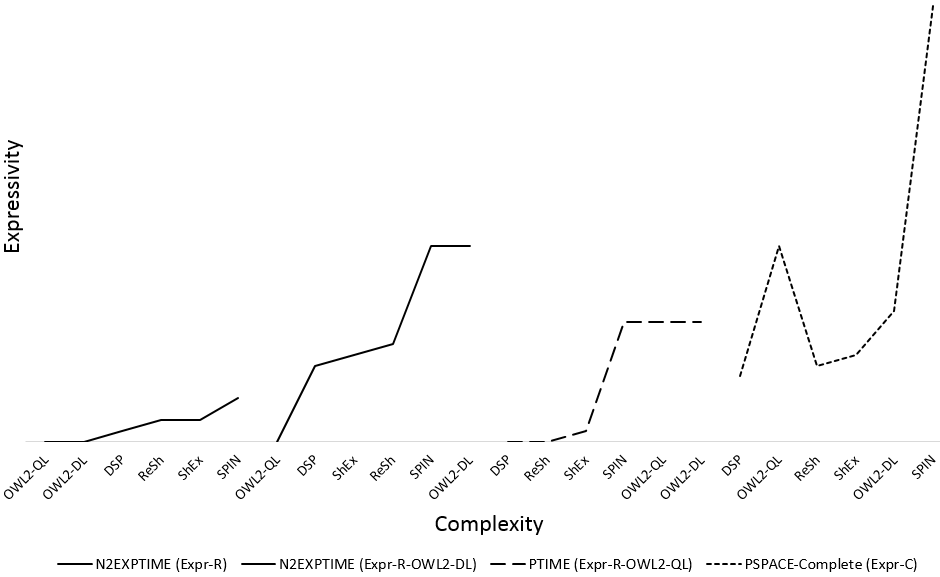
\includegraphics[width=1.00\textwidth]{expressivity-complexity-3.png}
	%\caption{Expressivity and Complexity}
	%\label{fig:expressivity-complexity}
%\end{figure}



%Expressivity and complexity classes can be combined in a diagram (see figure Figure~\ref{fig:expressivity-complexity}).

%\begin{figure}
	%\centering
		%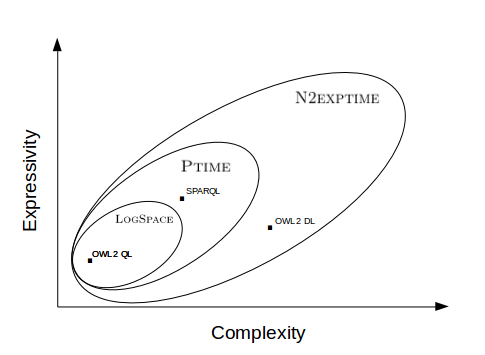
\includegraphics[width=0.95\textwidth]{complexiity_and_expressivity.png}
	%\caption{Complexity and Expressivity Classes}
	%\label{fig:expressivity-complexity}
%\end{figure}

%It depends on the individual use case, which constrains are needed to express and therefore which constraint language to choose.
%As a consequence, you may select a constraint language which is not the most expressive one within one specific expressivity class, 
%but may be better evaluated according to one or multiple user-friendliness classes.
%If, for instance, reasoning should not be performed and three particular constraints should be covered by the constraint language.
%Even if the absolute expressivity (\ms{Expr-C}) of SPIN is much higher than the one of ShEx (\ms{Expr-C}(ShEx) $\subset$ \ms{Expr-C}(SPIN)) 
%, the relative expressivity of this expressivity class could be the same for ShEx and SPIN - in case the three constraints are covered by both.
%\er{The expressivity here (in figure) is not constraint specific expressivity, it is more general. However, constraint specific expressivity must follow.}
%\tb{we need to create a new figure}
%Now, the user-friendliness classes comes into play:
%\begin{eqnarray*}
%\ms{UF-L}(SPIN) \subset \ms{UF-L}(ShEx), \ms{UF-I}(SPIN) \subset \ms{UF-I}(ShEx) \\
%\ms{UF-C}(SPIN) \subset \ms{UF-C}(ShEx), \ms{UF-L}(ShEx) \subset \ms{UF-L}(SPIN)
%\end{eqnarray*}
%Although, SPIN is more adopted than ShEx, ShEx is a high-level compared to a low-level language, ShEx is more intuitive and concise than SPIN.
%According to this evaluation, tools may recommend alternatives to the most expressive language SPIN.  

%\section{Implementation}
%\label{Implementation}
%
%SPARQL is generally seen as the method of choice to validate RDF data according to certain constraints, although it is not ideal for their formulation. 
%In contrast, OWL 2 DL constraints are comparatively easy to understand, but lack an implementation to validate RDF data. However, reasoning in OWL supports the identification of inconsistencies, which is also known as ontology debugging \cite{stuckenschmidt2008debugging}. Despite the fact that inconsistency detection especially in DL has already been studied extensively, it is not sufficient for constraint validation.
%Bosch and Eckert\cite{BoschEckert2014-2} use SPIN as basis to define a
%validation environment in which the validation of any constraint language\footnote{the only limitation is that constraint languages must be represented in RDF} can be implemented by representing them in SPARQL. 
%The validation implementation of constraint languages is fully declarative,
%consisting of a mapping from a constraint language to SPIN in form of SPARQL CONSTRUCT queries.
%SPIN represents both the SPIN mappings and the SPARQL queries in RDF. 
%Within the validation environment, we fully implemented the validation of all OWL 2 DL\footnote{and therefore all OWL 2 QL constructs} constructs. 
%The implementation can be tested at \url{http://purl.org/net/RDFval-demo} and
%the OWL 2 SPIN mapping is maintained at \url{https://github.com/boschthomas/OWL2-SPIN-Mapping}.
%
%The developed constraint language classification according to the three dimensions expressivity, complexity, and user-friendliness leads to many possible extensions of the RDF validator and similar validation systems.
%Users may choose if they wish to execute reasoning as a pre-validation step and which reasoning axioms they want to use to express their inference rules.
%They may also select which constraints they need for their use cases.
%
%As we defined an ordering of constraint languages for each expressivity class, we assigned reasoning axioms and constraints to complexity classes, we evaluated constraint languages regarding multiple user-friendliness criteria, the validator can provide a list of constraint languages for which the expressivity is enough to express the wished constraints and axioms.
%The validator can also recommend a constraint language of that list whose user-friendliness is evaluated to be the highest according to the user-friendliness criteria.
%As reasoning may cause high complexity, the validator may show which axioms from the user's selection cause the determined complexity class 
%and it may provide solutions how to get to the next lower complexity class.

\section{Related Work}
\label{sec:related-Work}

Tao \cite{tao2012integrity} proposed an OWL 2 DL extension to support integrity constraints and enables thereby the use of OWL as a constraint language for validation including the closed-world assumption. Beside a solution to explanation and repair of constraint violations, i.e. for integrity constraints, the author describes a sound and complete approach for constraint validation by conjunctive query answering.

Siren and Tao proposed an alternate semantics for OWL using CWA so that it could be used to validate integrity constraints.
This semantics is implemented in the Stardog database\footnote{\url{http://stardog.com/}}\cite{SirinTao2009}. 
They examined integrity constraint semantics proposed in the deductive databases literature and adopted them for OWL
by reducing the validation of integrity constraints to SPARQL query answering by means of reasoners.
This OWL semantics, however, was never submitted to a standards organization such as the W3C.

In description logics, reasoning tasks like query answering or detection of inconsistencies require the consideration of knowledge that is not only defined explicitly but also implicitly. To do so there are two different ways called forward- and backward-chaining. The first implies a materialized knowledge base, where the original knowledge base is extended by all assertions that can be inferred. State-of-the-art DL or OWL reasoners that following this approach are e.g. FaCT++ \cite{tsarkov2006fact++}, Pellet \cite{sirin2007pellet},  RacerPro \cite{haarslev2001racer}, or HermiT \cite{horrocks2012hermit}. On the second approach, the original knowledge base is kept in its original state and before queries are evaluated against the knowledge base, the queries will be rewritten such that its rewritings will consider also the implicit knowledge in the returned result set. Approaches following this way are e.g., \textsf{PerfectRef} given by Calvanese et al. \cite{Calvanese2007} or \textsf{TreeWitness} proposed by Kontchakov et al. \cite{kontchakov2011combined}. The choice between these two different ways depends on the specific application case. So the first kind is probably applied on local knowledge bases whereas the second is more appropriated for federative environments like in \cite{nolle2014efficient,nolle2013elite}.
\tb{2 papers, see following latex comments}
%Axel Polleres, Cristina Feier, and Andreas Harth. Rules with
%contextually scoped negation. In Proceedings of the 3rd European
%Semantic Web Conference (ESWC2006), volume 4011 of Lecture Notes in
%Computer Science (LNCS), pages 332-347, Budva, Montenegro, June 2006.
%Springer.
%
%And additionally:
%http://www2.informatik.uni-freiburg.de/~mschmidt/docs/sparql_constraints.pdf

\section{Conclusion and Future Work}

In section \ref{Expressivity-Complexity-OWL2} we explained why reasoning is beneficial for validation and how reasoning interacts with validation.
In section \ref{Classification-RDF-Constraints-Reasoning-Complexity} we classified RDF constraints according to reasoning and complexity.
We distinguish two disjoint constraint types $\mathcal{C}_{R}$ (constraints with reasoning) and $\overline{\mathcal{C}_{R}}$ (constraints without reasoning) to investigate the affect of reasoning to the validation process.
Regarding the performance of constraints, we refer to worst case complexity.
We divide $\mathcal{C}_R$ into two not disjoint classes ($\mathcal{C}_R ^{\mathcal{QL}} \subseteq \mathcal{C}_R ^{\mathcal{DL}}$) for the validation by query answering with OWL 2 QL and OWL 2 DL reasoning respectively.
It is well known known that performing SPARQL queries is in \textsc{Pspace}-Complete \cite{Perez2009}, 
which is assigned to $\overline{\mathcal{C}_R}$ (validation by query answering without reasoning).
In section \ref{Classification-Constraint-Languages-Expressivity-Complexity} we classified constraint languages according to expressivity. Later, we discussed briefly the important aspects of the friendliness of a constraint language, which would require a further investigation.
In sections 
\ref{sec:RDF-validation-requirements-and-reasoning} and
\ref{RDF-Validation-Requirements-without-Reasoning},
we present some constraints for each of the two constraint types $\mathcal{C}_{R}$ and $\overline{\mathcal{C}_{R}}$.
For $\mathcal{C}_{R}$ constraints we consider the effects of reasoning on validation.
We implemented the validation of all OWL 2 QL, OWL 2 DL, DSP (and the major ReSh and ShEx) constructs
within our SPIN validation environment in form of SPARQL CONSTRUCT queries (\url{http://purl.org/net/RDFval-demo}).
%\cite{BoschEckert2014-2}\footnote{SPIN mappings: \url{https://github.com/boschthomas/OWL2-SPIN-Mapping}, \url{https://github.com/dcmi/DSP-SPIN-Mapping}}.
For $\mathcal{C}_{R}$ constraint types (represented in OWL 2), you can choose if reasoning should be performed prior to validation.

As part of future work we extend the validator to provide a list of constraint languages for which the expressivity is enough to express selected constraints.
The validator may also recommend one of these constraint languages having the highest expressivity and lowest complexity.
As reasoning may cause high complexity, the validator may show which constraints from the user's selection cause the higher complexity class 
and it may provide solutions how to get to the next lower complexity class. In this regard, it would be charming to have an estimation on which group of constraints would demand what class of complexity. However, this is not an easy question, since complexity results are language specific and operational semantics is involved as well. Therefore, it is hard to maintain a general complexity result for a constraint independent of the language chosen. Yet, providing an estimation for particular cases can still be straightforward.

%\section{Christian's Feedback}
%
%everybody, in the following some comments related to the paper draft
%given to me by Erman. Feel free to include these comments. Further, I
%woul prefer to be removed from the authors list, because I do not have
%the time to work on the paper and I'm in the current status not so very
%happy with it. Anyhow, I think guys will be able to improve it. So here
%are now my comments.
%
%There are too many different issues that are not presented in a well
%structured way / partially overlapping In particular there are two main
%contributions for which it is hard to understand their interdependencies.
%
%a) the role of reasoning for constraint validation
%b) the classification of the 74 constraint pattern in relation to the 5
%constraint languages
%
%Honestly, i do not understand why there are certain paragraphs at
%certain places and how this all goes together. I discussed several
%details with erman and maybe he can put something into the paper.
%
%Anyhow, here are some suggestions that make the paper stronger. At the
%moment I have a feeling that there is only a low chance for acceptance,
%even though I see that lots of work is in this paper.
%
%1) I recommend to join section 1+2. In this new intro section I
%recommend to put an example for RDF validation, really oriented at a
%real scenario. For example, a library wants to publish some datasets as
%RDF by extracting them from different relational databases. In oder to
%achieve high data quality some constraints are defined first on a very
%generic level written down some natural language sentences.  Now it
%needs to be decided which formalism to use in order to formally express
%these constraints and to check their validity. Moreover, it needs to be
%clarified what role reasoning play in this verification and publication
%process. This will perfectly fit as motivation for the contribution of
%the paper and the example can be easily be used at other places of the
%paper.
%
%I would then always come back to the running example from the beginning
%and always use constraints that would fit to this scenario. I know you
%like this darth vader stuff, however, it is better to have some real
%usecase in mind otherwise people always think this is only relevant for
%such toy examples.
%
%2) I cannot see the difference between C_R and C_R' (i use ' instead of
%this complement line above). I think this not explained well and it
%would help a lot if there is one or better two examples from the 74
%constraint pattern for C_R and C_R'. However, there should also be a
%clear definition "C_R [are] constraints without reasoning" is not even a
%correct sentence, or differently speaking: The border of reasoning vs
%not reasoning is not well defined, there exists not such a border. I try
%to explain som of my problems.
%- The way I understand it, the distinction is based on whether a
%constraint is translatable to an OWL construct or not. The example with
%the Literal Pattern Matching seems to go in that direction.
%- If the criteria is whether or not its translateable to some formalims,
%then the table on bottom of page 8 makes no sense, especially the first
%column. This indicates whether a constraint belongs in one or the other
%class is independently of some chosen formalism
%- Is the Literal Pattern Matching an example for the C_R class? If yes
%its a very untypical one if you think of reasoning. Mayb it can be
%expressed with OWL, but is uses something very specific which looks very
%mud linke non reasoning.
%... after thinking a while I have a feeling that there is no real
%dictsinction between  C_R and C_R'.
%
%3) MAYBE: I recommend to remove the section on user friendliness. In a
%scientific paper this can only be answered by a field study or some
%questionaires or something like this.
%
%4) The UNA and CWA are important aspects, however, in Section 4 nd 5
%they are not used anymore. I would expect that a constraint type can be
%independent of the CWA or it can make a difference. For example:
%
%ex1: An address is a field that stores a string and its end is substring
%that refers to a number.
%ex2: If someone is a mother, she has at least one child.
%ex3: If someone is a women, it cannot be a man.
%
%ex1 has nothing to do with CWA or UNA, if you accept the CWA or its
%opposite, it doe not nmake a difference here.
%ex2 depends on CWA, in the CWA setting a mother without an explictly
%stated child violates the constraint. In OWA its different, the mother
%withour explicitly stated child is not a problem. You just have an axiom
%that allows you to entail that there is an (unknown) child.
%ex3 again independent of CWA.
%
%I was really wondering how many of the 74 patterns are independent and
%how many are dependent? Note that you can give a very clear definition
%what independent means. You can say, For a given constraint, if there
%exist not RDF dataset that would be inconsistent under CWA and
%consistent under OWA or vice versa, then the constraint is independent
%of the CWA.
%
%5) Make the tables floating such that the have figure caption andnnumber
%and refer to these numbers from the text
%
%6) You should discuss the argumenst in Section 7 in the light of the
%library example given in he intro. The argumentation in this section is
%somewhat strange because this seems to touch the question whether to
%materialize explict or to keep tjis implicit. It is also strange why
%eactly the spefic constructs listed in the subsctions have been picked.
%
%... the last pages of the paper I have not been reading in details and I
%will not find the time to do this.
%
%This might be worth reading, the hint was just given from Heiner:
%
%Axel Polleres, Cristina Feier, and Andreas Harth. Rules with
%contextually scoped negation. In Proceedings of the 3rd European
%Semantic Web Conference (ESWC2006), volume 4011 of Lecture Notes in
%Computer Science (LNCS), pages 332-347, Budva, Montenegro, June 2006.
%Springer.
%
%And additionally:
%http://www2.informatik.uni-freiburg.de/~mschmidt/docs/sparql_constraints.pdf
%
%Best regards, Christian.


\bibliography{../../literature/literature}{}
\bibliographystyle{plain}
\setcounter{tocdepth}{1}
%\listoftodos
\end{document}
